\documentclass[11pt]{article}
\usepackage[a4paper,margin=2.5cm]{geometry}
\usepackage[T1]{fontenc}
\usepackage{amsmath}
\usepackage{newtxtext,newtxmath} % provides the amssymb symbols; amssymb itself clashes with newtxmath
\usepackage[varqu,scaled=0.95]{zi4} % scalable typewriter font (Inconsolata) for code
\usepackage{graphicx}
\usepackage{booktabs,array,makecell,rotating}
\usepackage[authoryear,round]{natbib}
\usepackage{xurl} % loads url; paths may break at any character
\usepackage{xcolor}
\usepackage{microtype}
\usepackage{caption}
\usepackage{siunitx}
\usepackage{enumitem,needspace}
\usepackage[hidelinks]{hyperref}
\hypersetup{pdftitle={Workers of large-colony ants do not have smaller brains: a preregistered test},pdfauthor={}}

%%%%% Math commands used in the ANT-TWIN preprint (only those that are used) %%%%%

% Logarithm to base 10, used for all volumes and colony sizes.
\newcommand{\lten}{\log_{10}}

% Normal distribution; Pagel-lambda transformed phylogenetic covariance; MCC correlation matrix.
\newcommand{\Normal}{\mathcal{N}}
\newcommand{\Clam}{\mathbf{C}_{\lambda}}
\newcommand{\Amat}{\mathbf{A}}

% Covariate vector of the measurement-error model.
\newcommand{\vx}{\mathbf{x}}

% Scan-step indicator of the primary model, e.g. \Step{1.22}.
\newcommand{\Step}[1]{\mathrm{Step}_{#1}}

% Body volume of the owners' program at a given threshold, e.g. \body{110}.
\newcommand{\body}[1]{\mathrm{body}(#1)}

% Standard error and intraclass correlation.
\newcommand{\SE}{\mathrm{SE}}
\newcommand{\ICC}{\mathrm{ICC}(1)}


\captionsetup{font=small,labelfont=bf,labelsep=period}
\sisetup{range-phrase=--,range-units=single}
\urlstyle{tt}
\setlength{\emergencystretch}{1.5em}
% Float placement: allow tall top floats; a float page only for floats that nearly fill it.
\renewcommand{\topfraction}{0.85}
\renewcommand{\textfraction}{0.1}
\renewcommand{\floatpagefraction}{0.7}

\newcommand{\marker}[1]{\textcolor{red}{#1}}

\title{Workers of large-colony ants do not have smaller brains:\\a preregistered test}
\author{Daglar Dragomirov\\[2pt]
\normalsize Saint Petersburg State University, Saint Petersburg, Russia\\
\normalsize \href{mailto:daglar.dragomirov@gmail.com}{daglar.dragomirov@gmail.com}\\
\normalsize ORCID: \href{https://orcid.org/0009-0003-6110-4188}{0009-0003-6110-4188}}
\date{}

\begin{document}
\maketitle

\begin{abstract}
Large insect societies make many decisions collectively, which could relax cognitive demands on individual workers
and favour smaller brains (the distributed-cognition hypothesis); the social-brain hypothesis predicts the opposite.
We tested these predictions in $270$ ant species with a preregistered phylogenetic model, using worker brains
segmented automatically from AntScan synchrotron micro-CT scans and checked by a vision-language-model agent.
Relative brain volume increased with colony size. The increase was about $8\%$ per tenfold increase in colony size,
and the $95\%$ confidence interval excluded zero, which met the preregistered criterion for the social-brain
hypothesis. The result held across posterior trees, a second phylogeny, a model of measurement error and all
robustness checks except the soft-tissue denominator. Exploratory analyses showed that the effect size depends on the
body measure: with independently measured body volumes, or with soft tissue (body minus cuticle), it shrank to a
small, uncertain value. Thinner cuticle in large-colony species explained only a small part of this difference; most
of it traced to errors in a few of our own body masks. In every analysis in Table~\ref{tab:robustness}, estimates were
positive and intervals excluded a decrease as large as the preregistered smallest effect of interest. Taken together,
our results show that workers of large-colony species do not have smaller brains: brain investment is maintained or
at most modestly increased.
\end{abstract}

\begin{small}
\noindent\textbf{Keywords:} ants, brain size, colony size, social brain hypothesis, distributed cognition, micro-CT,
deep learning, phylogenetic comparative methods, preregistration

\end{small}

\section{Introduction}\label{sec:intro}

Colony size varies widely in ants: species range from colonies of a few workers to millions, and in our data set
species means span $7$ to $10^{7}$ workers. It evolves gradually across the ant phylogeny~\citep{burchill2016}, and
group size shapes how colonies are organised, including division of labour and collective
decision-making~\citep{dornhaus2012}. A precedent comes from cuticle: across ants, workers of species with larger
colonies invest less in cuticle. \citet{matte2025} described these as ``cheaper workers'' and argued that this
facilitated larger societies. This finding raises a direct question: is the per-worker economy limited to protective
tissue, or does it extend to neural tissue? Two classic ideas give opposite answers. Under the distributed-cognition
hypothesis (H1), information processing in large colonies is spread across many workers, so each worker may need less
individual processing~\citep{feinerman2016,odonnell2015}. Selection could then reduce its brain investment. The
social-brain hypothesis (H2) predicts the opposite, because larger and more complex societies may demand more
processing of social information from each member~\citep{dunbar1998,gronenberg2009,lihoreau2012}.

The evidence so far comes from few species, mostly within one genus or tribe, and some studies examined specific
neuropils rather than total brain volume (Section~\ref{sec:related}). To our knowledge, no study has tested colony
size against worker brain size across hundreds of ant species within a phylogenetic framework.

We ask whether workers of species with larger colonies have smaller brains for their body size. Our answer is that
they do not: across $270$ species, the distributed-cognition prediction of smaller brains was not supported by any
analysis. The preregistered test instead found a positive association, but its magnitude depends on how body volume
is measured.

AntScan, a synchrotron micro-CT survey of ant specimens that spans $792$ species~\citep{katzke2026}, allows brain
volumes to be measured across species at a scale that manual segmentation cannot reach. On these scans we built an
automated pipeline of brain localisation, nnU-Net segmentation~\citep{isensee2021} and vision-agent quality control,
and froze the resulting brain table. Figure~\ref{fig:scan} shows this pipeline on real scans, from the whole specimen
to the brain mask, and Supplementary Figure~\ref{fig:schematic} gives a schematic of the measurement and analysis
pipeline. We then preregistered one primary test of the colony-size slope, with a smallest effect size of interest
(SESOI) and explicit decision rules, and ran the preregistered robustness checks. Exploratory analyses separated brain
investment relative to soft tissue from investment relative to total body volume. Figure~\ref{fig:forest} shows the
colony-size estimate in the primary analysis and in every robustness check.

\begin{figure}[tbp]
\centering
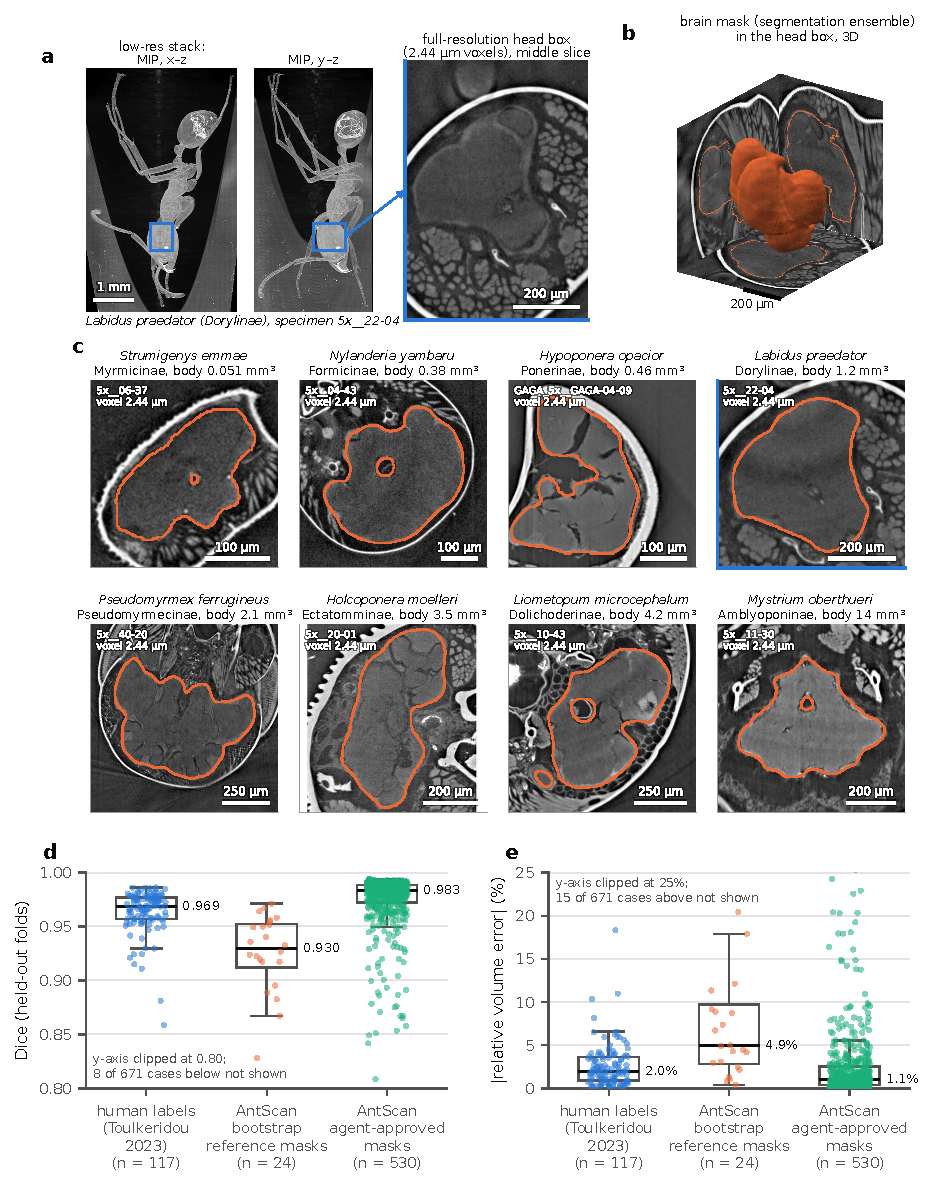
\includegraphics[width=0.8\textwidth]{figures/fig1_scan_to_brain.pdf}
\captionsetup{font=footnotesize}
\caption[From scan to brain volume]{\textbf{From scan to brain volume.} Panels a--c show the automated pipeline on
real AntScan scans; d--e show its held-out accuracy.
\textbf{(a)}~One specimen through brain localisation (\emph{Labidus praedator}, Dorylinae, specimen
\path{5x__22-04}). Left: maximum-intensity projections (MIP) of the AntScan low-resolution copy that the head finder reads
(here \qty{4.9}{\um} between slices, \qty{9.4}{\um} in plane), with the full-resolution head box (blue) at the
coordinates of the box; for this specimen the box had been regrown (Section~\ref{sec:brain}). The ant hangs
head-down in the vial. Right: middle slice of the head box at full resolution (\qty{2.44}{\um} voxels).
\textbf{(b)}~The brain mask of the same specimen (segmentation ensemble, as frozen) as a surface inside its head box. The
three orthogonal box slices through the mask centroid are drawn on the back walls with the mask outline. Orthographic
view; for display only, the surface was computed on the mask downsampled twofold and smoothed. The scale bar lies
along the front edge of the box floor.
\textbf{(c)}~Brain masks of eight specimens from the frozen brain table, shown without edits. Each tile shows the scan
slice with the largest brain cross-section in the full-resolution head box, with the mask outline (orange) and a scale
bar; the crop is centred on the mask, and white areas lie outside the box. Titles give species, subfamily and
body volume (owner-measured or from our body masks; Section~\ref{sec:body}); the specimen code and voxel size are
printed in each tile. \emph{Selection rule:} the pool was
the $462$ main-analysis workers with a body volume, split into octiles of $\lten$ body volume. From the smallest
octile up, one specimen was drawn at random (NumPy \texttt{default\_rng}, seed 20261116) among pool workers of
subfamilies not yet drawn, so the eight specimens come from eight subfamilies. All eight happen to be \qty{2.44}{\um}
scans, the voxel class of $398$ of the $462$ pool workers. The specimen of panels a--b, framed in blue, is the drawn
specimen closest to the pool median body volume.
\textbf{(d)}~Dice and \textbf{(e)}~$|$relative volume error$|$ of our segmentation model on held-out folds
(species-level folds within each source), by reference type: human labels of \citet{toulkeridou2023}, $n = 117$;
AntScan bootstrap reference masks, $n = 24$; agent-approved AntScan masks, $n = 530$ (produced by an earlier model,
hence not independent). Boxes show quartiles; numbers are medians. Axes are clipped: $8$ cases below Dice $0.80$ and
$15$ above $25\%$ error are not shown. Inputs are listed in the code repository's storage index.}
\label{fig:scan}
\end{figure}

To test this claim, we ask three questions.
\begin{itemize}
\item[\textbf{Q1}] \emph{Are the automated brain volumes accurate enough for a comparative test?} Yes: segmentation
matched held-out human labels closely, brain volume was repeatable within species, and both preregistered gates were
passed (Section~\ref{sec:q1}).
\item[\textbf{Q2}] \emph{Do workers of large-colony species have smaller brains for their body size?} No: in the
preregistered test, relative brain volume increased with colony size, and all preregistered robustness checks except
the soft-tissue denominator gave the same outcome (Section~\ref{sec:q2}).
\item[\textbf{Q3}] \emph{Does the estimate depend on how body size is measured?} Yes: with the most accurate size
measures, the estimate shrank to a small, uncertain value, and thinner cuticle explained only a small part of the
difference (Section~\ref{sec:q3}).
\end{itemize}

\paragraph{Contributions.} This paper makes three contributions.
\begin{itemize}
\item \textbf{A comparative data set of worker brain volumes.} We measured brain volume automatically in workers of
$325$ species, with segmentation validated against human labels and every mask reviewed by a vision-language-model
agent (Sections~\ref{sec:brain} and~\ref{sec:q1}).
\item \textbf{A preregistered phylogenetic test of the colony-size prediction.} Colony size was tested against relative
brain volume with a smallest effect size of interest and decision rules fixed before unblinding
(Sections~\ref{sec:model} and~\ref{sec:q2}).
\item \textbf{A decomposition by body-size measure.} Measuring body and soft tissue with the same instrument on the
same specimens separates the contribution of thinner cuticle from differences between body-volume sources
(Section~\ref{sec:q3}).
\end{itemize}

Section~\ref{sec:related} relates the two hypotheses to earlier tests, and Section~\ref{sec:methods} describes the
measurements and the analysis plan. The three questions are answered in Section~\ref{sec:results}, and
Section~\ref{sec:discussion} discusses what the results do and do not show.

\subsection{Related work: two hypotheses and earlier tests}\label{sec:related}

\paragraph{Distributed cognition and the cost of neural tissue.} Neural tissue is metabolically
expensive~\citep{aiello1995,niven2008}, so selection could reduce brain investment when the colony takes over part of
the computation. In vespid wasps, mushroom-body investment fell at the origins of sociality~\citep{odonnell2015}.
Among fungus-growing ants, relative brain size was smaller in monomorphic species with large
colonies~\citep{riveros2012}. Unlike these studies within single clades, we test the prediction on whole-brain volume
across $270$ species from $12$ subfamilies.

\paragraph{Social brains in ants.} Some comparisons in ants point towards the social-brain prediction. Within
\emph{Cataglyphis}, species with larger colonies have larger brains~\citep{wehner2007}, and socially complex
\emph{Oecophylla} invests more in brain tissue than \emph{Formica}~\citep{kamhi2016}. Rather than comparing species
within one genus or two genera, we estimate the colony-size slope across the family in a phylogenetic model with a
preregistered smallest effect of interest.

\paragraph{Direct tests of colony size and brain size.} Such tests used few species, for example
$2$~\citep{kamhi2016}, $3$~\citep{godfrey2020} or $18$~\citep{riveros2012}, mostly within one genus or tribe. In
harvester ants (\emph{Pogonomyrmex}), species with larger colonies did not have larger brains~\citep{perl2026}. Other
work examined specific neuropils, such as antennal lobes, rather than total brain
volume~\citep{godfrey2020,marty2025}. In contrast, we measure total brain volume in workers of hundreds of species
from the AntScan survey.

\paragraph{Cheaper workers.} Most closely related to our work is the comparative study of cuticle investment by
\citet{matte2025}, who measured body and cuticle volumes on AntScan specimens and used the same phylogeny. Unlike
\citet{matte2025}, whose measurements concern protective tissue, we measure investment in neural tissue and use their
body and cuticle measurements as size denominators.

\section{Methods}\label{sec:methods}

\subsection{Study design and specimens}\label{sec:design}

Our comparison combines four quantities: species means of worker brain volume and body volume, the colony size of
each species, and its position on the ant phylogeny. We use the term \emph{relative brain volume} for brain volume at
equal body volume, stain and scan step. Accordingly, we write $\beta_2$ for the colony-size slope, the change in
$\lten$ brain volume per $\lten$ unit of colony size at equal body volume, stain and scan step. By \emph{soft tissue}
we mean body volume minus cuticle volume.

Specimens come from AntScan, synchrotron micro-computed tomography (micro-CT) scans made at the Karlsruhe Institute of
Technology (KIT). The scans are hosted on Biomedisa under a Creative Commons Attribution licence (CC BY 4.0;
\citealp{katzke2026}; \citealp{losel2020}). The target set comprised all colony workers (caste ``worker'' in the
AntScan metadata) of species with a species-level colony size: $818$ specimens of $352$ species. Scans differ in voxel
size (1.22, 2.44 or \qty{6.11}{\um}; \qty{8.2}{\um} was merged with \qty{6.11}{\um}) and in staining (iodine or
unstained). Both are partly confounded with body size, so both enter the model as covariates
(Section~\ref{sec:model}). Appendix~\ref{app:impl} describes how scan stacks were read.

\subsection{Brain volume: localisation, segmentation and quality control}\label{sec:brain}

\paragraph{Localisation and segmentation.} The brain pipeline has three steps: localisation, segmentation and quality
control. First, a low-resolution head finder (nnU-Net 3d, trained on $471$ of $497$ approved low-resolution brains,
resampled to isotropic \qty{12}{\um} and cropped to the specimen) located the brain in each specimen. A
full-resolution box was then cut around the head (Figure~\ref{fig:scan}a); boxes that cut off part of the brain were
regrown, and unresolved cases received second and third finder candidates. Brains were then segmented with our
segmentation model, a 5-fold nnU-Net 2d ensemble (hereafter the segmentation ensemble) trained on three sources:
\begin{itemize}[nosep]
\item $117$ micro-CT stacks with human brain labels from \citet{toulkeridou2023};
\item $24$ AntScan brains with bootstrap reference masks, that is, automatic draft masks approved by vision agents in a
first review round;
\item $530$ AntScan brains approved by vision-agent quality control in earlier rounds.
\end{itemize}
Folds were assigned by species within each data source, and the final segmentation of every specimen is the 5-fold
ensemble without test-time augmentation (Figure~\ref{fig:scan}b--c). Accuracy was assessed on the held-out folds
against each kind of reference (Section~\ref{sec:q1}). ``Brain'' is the structure delineated in the reference labels of \citet{toulkeridou2023}: the nervous
tissue of the head capsule segmented as one object, including the subesophageal zone, which in ants is fused with the
brain. All masks follow this definition, so it applies equally to every species and cannot bias the comparison among
them; absolute volumes may differ from studies that exclude the subesophageal zone.

\paragraph{Quality control (QC).} No human reviewed the masks. Instead, every final mask was reviewed by a multimodal
language-model agent (Claude Opus 5.5, Anthropic; high reasoning effort). It saw a contact sheet of eight slices
through the head box, with the mask outline overlaid. The agent judged whether the box is on the head, whether the
mask is good, needs fixing or is bad, and whether the brain lies fully inside the box, and it estimated the volume
error. A specimen entered the brain table only with ``mask good'', ``box on head'' and ``brain fully in box'';
Supplementary Figure~\ref{fig:qcrej} shows rejected masks with the agent's verdicts. Verdicts, prompts and images are
archived (\hyperref[sec:data]{\emph{Data and code availability statement}}), and the table was frozen before
unblinding (checksum in Appendix~\ref{app:impl}).

\subsection{Body volume and soft tissue}\label{sec:body}

\paragraph{Body volume.} This preregistered primary size covariate came from two sources, in this order. Where a
specimen had been measured by \citet{matte2025}, we used their individual measurement (their Dataset S1; hereafter
owner-measured volumes). Otherwise we used our own body mask: a three-class multi-Otsu segmentation inside the
vial, with per-slice contour closing and filling, and correct slice spacing from the true number of slices
(Appendix~\ref{app:impl}). These masks
agreed with the owner-measured volumes with a median ratio of $1.04$ ($n = 278$ specimens), and specimens with $20$ or
more ``guarded'' slices (bright mounting medium) had no valid body volume. Of the $462$ main-analysis workers with a
body volume, $235$ had owner-measured values and $227$ had values from our masks.

\paragraph{Soft tissue.} Robustness check R3 used owner-measured soft tissue, available for $154$ of the $270$ primary
species. The preregistration anticipated adding our own cuticle measurements ``if time permits'', and we did so in an
extension declared after unblinding. For this extension we ran the owners' own segmentation program
(\citealp{matte2025}; Zenodo record 15546461, CC BY 4.0) unchanged on $185$ specimens. These were $141$ target workers
(at most two per species) from the $116$ primary species without owner-measured soft tissue, and $44$ owner-measured
specimens for validation.

\paragraph{Subsampled slices.} Because the AntScan server throttles downloads, only the slices actually used were
read, by HTTP range requests: every third slice, plus every thirtieth slice for the program's $z$-limit search. The
program's median filter therefore spans $9$ sampled slices instead of $25$. On $8$ specimens processed at every slice,
the ratio of every-third-slice to every-slice volumes had a median of $0.9996$ for body (range 0.990--1.010; $7$
specimens, since one bright-medium scan has no body mask at threshold $110$). For soft
tissue, the median was $0.9991$ (range 0.978--1.002).

\paragraph{Threshold rules.} With the authors' threshold ($110$), a bright mounting medium leaks into the mask in many
scans, and the authors' scripts contain both $110$ and $145$. Our main (``adaptive'') rule therefore used threshold
$110$ if $\body{110}/\body{130}$ lay within $1/1.10$--$1.10$ and otherwise $145$ if $\body{145}/\body{130}$ lay within
that range. Specimens that met neither condition were excluded (Supplementary Figure~\ref{fig:cuticle}), and in all
cases the rule required cuticle/body between $0.03$ and $0.40$. A ``strict'' rule, used as a sensitivity analysis,
allowed threshold $110$ only, with body volume stable across all three thresholds ($\max/\min \le 1.15$). The adaptive
rule passed $141$ of $185$ specimens (threshold $110$: $92$; threshold $145$: $49$), and the strict rule passed $88$.

\paragraph{Validation.} Of the $44$ validation specimens, the adaptive rule accepted $41$. On these, our measurements
reproduce the owners' values, with median ratios of $0.998$ for body, $1.04$ for cuticle and $0.992$ for soft tissue.
The correlation of log soft tissue was $r = 0.997$, and the three excluded validation specimens are the ones that
disagree with the owner-measured values.

\subsection{Colony size and phylogeny}\label{sec:colony}

\paragraph{Colony size.} Species colony size is the geometric mean of the mean nest sizes recorded in Dataset S3 of
\citet{matte2025}. For species without S3 records, we used the colony size from \citet{bellroberts2024}; this applied
to $6$ of the $270$ primary species. Across the $270$ primary species, colony size ranges from $7$ to $10^{7}$ workers
(median $300$; SD of $\lten$ colony size $1.24$).

\paragraph{Phylogeny.} The primary tree is the maximum-clade-credibility (MCC) tree of the \citet{economo2018}
${\sim}15{,}000$-species phylogeny (NC-uniform, stem); \citet{matte2025} used the same phylogeny (mean covariance of
its FBD trees). Tree uncertainty was assessed on $100$ NC-stem posterior trees (preregistered). Alternative trees were
$200$ FBD crown and stem posterior trees (check R1) and the genus-level dated phylogeny of \citet{borowiec2025}
(check R2). Species were placed on the tree by exact name, then subspecies, then a fixed list of post-2018 genus
transfers, and then a free tip of the same genus. Of the $270$ primary species, $257$ matched by exact name, $12$ via
genus transfer and $1$ by genus placement.

\subsection{What was fixed before unblinding, and what was not}\label{sec:prereg}

The analysis plan and outcome rules were preregistered (OSF ``secondary data analysis'' template) as version 0.1
on 13 November 2026. The plan was frozen, with declared deviations, on 15 November 2026,
before any model containing colony size was fitted to real brain volumes (commit and tag in Appendix~\ref{app:impl}).
Measurement stages never read the colony table, and until the freeze, analysis runs wrote only a ``has colony'' flag
next to brain values. The deviations declared at the freeze concern the segmentation model, mask review by vision
agents instead of humans, and body volumes from corrected body masks instead of an earlier version of the body masks.
They also concern registration as a
timestamped GitHub commit and tag instead of OSF, and running the measurement-error model after the primary test.
After unblinding, the measurement protocol and QC rule of the soft-tissue extension were specified; the rule was fixed
before the final fits and revised once, on segmentation diagnostics. An interim estimate on $28$ added species
($+0.007$) had been seen before that rule was written, so both rule versions are reported. Appendix~\ref{app:dev}
lists every deviation. Finally, the test concerns the whole-brain volume of minor and monomorphic workers; it does not
address brain composition, such as the mushroom bodies.

\subsection{Statistical model and decision rules}\label{sec:model}

\paragraph{Worker selection.} Species values are means of $\lten$ volumes over workers of one preparation that passed
quality control: unstained workers if any, otherwise iodine-stained ones, and the modal scan-step class. Only minor
and monomorphic workers were used, so major, media and intercaste workers were excluded, as were workers with damage
that affects the brain (head or anterior truncation, oversaturation, badly preserved soft tissue).

\paragraph{Primary model.} The primary model is a phylogenetic generalised least squares (PGLS) regression of $\lten$
brain volume on $\lten$ body volume, $\lten$ colony size, stain and scan step:
\begin{equation}\label{eq:pgls}
\begin{split}
\lten\mathrm{Brain} &= \beta_0 + \beta_1\lten\mathrm{Body} + \beta_2\lten\mathrm{Colony} + \beta_3\,\mathrm{Iodine}
  + \beta_4\Step{1.22} + \beta_5\Step{6.11} + \varepsilon,\\
\varepsilon &\sim \Normal\bigl(0,\sigma^2\Clam\bigr).
\end{split}
\end{equation}
In words, $\beta_1$ is the brain--body slope, $\beta_2$ the colony-size slope, and $\beta_3$ to $\beta_5$ adjust for
staining and scan step. Here $\Clam$ is the Pagel-$\lambda$ transformed MCC covariance~\citep{pagel1999,freckleton2002},
with $\lambda$ estimated by maximum likelihood; $95\%$ CIs for $\beta_2$ are $t$-intervals with $n - 6$ degrees of
freedom. We fitted model~\eqref{eq:pgls} with our own Python implementation and cross-checked it against
\texttt{phylolm}~\citep{ho2014} and \texttt{nlme::gls(corPagel)}; differences were below $10^{-6}$. For tree
uncertainty, the model was refitted on the $100$ posterior trees and summarised by the median and a pooled interval (a
mixture of the per-tree $t$ sampling distributions).

\paragraph{Gates before unblinding.} Before unblinding, the data had to pass two gates. The Haller's-rule positive
control, a PGLS-$\lambda$ fit of $\lten$ brain on $\lten$ body, stain and scan step, required a slope in
$[0.4, 0.9]$, a CI inside $(0, 1)$ and $R^2 > 0.5$. In the synthetic-recovery gate, brains were simulated on the real
tree, species set and colony sizes with $\beta_2 = -0.03$ ($200$ replicates).

\paragraph{Sample size and precision.} The sample was fixed by data availability: every AntScan species with colony
size, an approved brain, body volume and a tip in the tree (expected 310--340 species in the preregistration; $270$
realised). The preregistration justified this size by simulation on the real MCC tree and colony sizes
($\lambda = 0.8$, brain--body slope $0.7$, measurement noise $0.03$ $\lten$, $1000$ replicates; Supplementary
Table~\ref{tab:S10}). With a species-level residual SD of 0.10--0.15 the expected $\SE(\beta_2)$ was 0.004--0.006,
giving a power of at least $0.91$ to detect $\beta_2 = -0.02$ and of at least $0.93$ to declare equivalence within
$\pm 0.02$ when $\beta_2 = 0$; with a residual SD of $0.25$ (SE $0.010$) these powers fall to $0.53$ and $0.33$. The
synthetic-recovery gate on the realised species set confirmed unbiased recovery (see Results). In the real data the
SE of $\beta_2$ was $0.0094$ ($n = 270$), so the half-width of the $95\%$ CI (about $0.018$) is smaller than the
SESOI: the design resolves effects of the size of the SESOI, and an interval that excludes $-0.02$ reflects the data
rather than low precision.

\paragraph{Decision rules.} The smallest effect size of interest was $|\beta_2| = 0.02$, about $4.7\%$ brain volume
per tenfold difference in colony size. Outcomes were labelled as follows, where $[L_{95}, U_{95}]$ and
$[L_{90}, U_{90}]$ denote the $95\%$ and $90\%$ intervals of $\beta_2$.
\begin{center}
\small
\begin{tabular}{@{}l>{\raggedright\arraybackslash}p{0.76\linewidth}@{}}
\toprule
Outcome & Condition \\
\midrule
Support H1 & $95\%$ CI entirely below $0$: $U_{95} < 0$ \\
Support H2 & $95\%$ CI entirely above $0$: $L_{95} > 0$ \\
Equivalence (H0) & $90\%$ CI inside $(-0.02, 0.02)$: $-0.02 < L_{90}$ and $U_{90} < 0.02$; a two one-sided
  test~\citep{lakens2017} \\
Small but non-zero & CI excludes $0$ and lies inside $\pm 0.02$ \\
Undecided & otherwise \\
\bottomrule
\end{tabular}
\end{center}
The label ``robust'' is added if the posterior-tree interval gives the same outcome and the measurement-error model
does not contradict it.

\subsection{Robustness checks and exploratory analyses}\label{sec:robust}

\paragraph{Preregistered robustness checks.} The $14$ preregistered robustness checks R1--R14 vary the phylogeny, the
size measure, the species and worker sets, the colony-size measure and the phylogenetic model
(Table~\ref{tab:robustness}):
\begin{center}
\small
\begin{tabular}{@{}l>{\raggedright\arraybackslash}p{0.86\linewidth}@{}}
\toprule
Check & Variant \\
\midrule
R1 & FBD posterior trees \\
R2 & \citet{borowiec2025} tree, one random species per genus, $100$ resamples \\
R3 & Soft tissue instead of body volume \\
R4 & Leaving out each subfamily with $\ge 10$ species \\
R5 & Unstained species only \\
R6 & All workers, including majors \\
R7 & Without names qualified by cf./aff./nr. \\
R8 & Without supercolonial species and social parasites~\citep[Supplementary Table~21]{bellroberts2024} \\
R9 & Colony size from \citet{bellroberts2024} only, or the maximum instead of the mean \\
R10 & Genus-level colony size \\
R11 & Without genus-placed tips \\
R12 & $\lambda = 1$, and the owners' method: mean covariance of FBD trees divided by $200$ as a fixed correlation \\
R13 & Badly preserved specimens returned, with collection year as a covariate \\
R14 & OLS without phylogeny \\
\bottomrule
\end{tabular}
\end{center}
Appendix~\ref{app:impl} gives the implementation details of R2 and R8.

\begin{sidewaystable}
\centering
\caption[$\beta_2$ in the primary analysis and all robustness checks]{\textbf{$\boldsymbol{\beta_2}$ ($\lten$ colony
size) in the primary analysis and all robustness checks.} Outcome labels follow the preregistered decision rules (Section~7 of the preregistration): support H2 = $95\%$ CI $> 0$; support H1 = $95\%$ CI $< 0$; equivalence = $90\%$ CI inside $(-0.02;\,0.02)$; otherwise undecided. $90\%$ intervals for single fits are $t$-intervals with $n - 6$ df. For tree sets and resamples, $\beta_2$ is the median and the interval is the pooled $t$-mixture interval. `Post hoc check' rows were computed after the preregistered analyses.
Trees: number of trees or resamples, and share: the share of them with $p < 0.05$ (tree sets and resamples only).}
\label{tab:robustness}
\fontsize{7}{8}\selectfont
\setlength{\tabcolsep}{3pt}
\begin{tabular}{@{}l>{\raggedright\arraybackslash}p{9.0cm}>{\raggedright\arraybackslash}p{1.9cm}rrccrrrrl@{}}
\toprule
ID & Check & Preregistered & $n$ & $\beta_2$ & $95\%$ CI & $90\%$ CI & $p$ & $\lambda$ & Trees & Share & Outcome \\
\midrule
P & Primary: PGLS-$\lambda$, Economo 2018 MCC tree & yes & 270 & $+0.035$ & $[+0.017;\,+0.054]$ & $[+0.020;\,+0.051]$ & 0.0002 & 0.72 &  &  & support H2 \\
P-post & Primary over 100 NC-stem posterior trees & yes & 270 & $+0.033$ & $[+0.014;\,+0.051]$ & $[+0.017;\,+0.048]$ &  & 0.64 & 100 & 1.00 & support H2 \\
ME & Measurement-error model, brms ($m = 0.0311$; specimen level, 442 specimens; posterior mean, CrI) & yes & 270 & $+0.038$ & $[+0.019;\,+0.055]$ & $[+0.023;\,+0.053]$ &  &  &  &  & support H2 \\
ME-tk & Measurement-error model, brms, $m = 0.0127$ (sensitivity) & yes & 270 & $+0.038$ & $[+0.020;\,+0.056]$ & $[+0.022;\,+0.053]$ &  &  &  &  & support H2 \\
ME-mcmc & Measurement-error model, MCMCglmm cross-check (posterior mean, 95\% CrI) & yes (fallback) & 270 & $+0.038$ & $[+0.020;\,+0.056]$ &  &  &  &  &  & support H2 \\
\midrule
R1 & R1 FBD posterior trees as run (3 crown + 3 stem) & yes & 270 & $+0.032$ & $[+0.014;\,+0.051]$ & $[+0.017;\,+0.047]$ &  & 0.59 & 6 & 1.00 & support H2 \\
R1-200 & R1 all 200 FBD posterior trees (post hoc check) & post hoc check & 270 & $+0.032$ & $[+0.014;\,+0.051]$ & $[+0.017;\,+0.048]$ &  & 0.60 & 200 & 1.00 & support H2 \\
R2 & R2 Borowiec 2025 tree, one random species per genus, 117 genera & yes & 117 & $+0.029$ & $[+0.001;\,+0.058]$ & $[+0.005;\,+0.054]$ &  & 0.50 & 100 & 0.77 & support H2 \\
R3 & R3 soft tissue (S1 body $-$ cuticle) as size measure & yes & 154 & $+0.006$ & $[-0.013;\,+0.024]$ & $[-0.010;\,+0.021]$ & 0.5576 & 0.00 &  &  & undecided \\
R4 & R4 without Dolichoderinae & yes & 258 & $+0.038$ & $[+0.019;\,+0.058]$ & $[+0.022;\,+0.054]$ & 0.0001 & 0.73 &  &  & support H2 \\
R4 & R4 without Dorylinae & yes & 260 & $+0.036$ & $[+0.016;\,+0.055]$ & $[+0.019;\,+0.052]$ & 0.0004 & 0.74 &  &  & support H2 \\
R4 & R4 without Formicinae & yes & 214 & $+0.024$ & $[+0.003;\,+0.045]$ & $[+0.007;\,+0.042]$ & 0.0225 & 0.72 &  &  & support H2 \\
R4 & R4 without Myrmicinae & yes & 149 & $+0.042$ & $[+0.013;\,+0.071]$ & $[+0.018;\,+0.066]$ & 0.0051 & 0.60 &  &  & support H2 \\
R4 & R4 without Ponerinae & yes & 221 & $+0.038$ & $[+0.020;\,+0.055]$ & $[+0.023;\,+0.053]$ & $<$0.0001 & 0.72 &  &  & support H2 \\
R5 & R5 unstained species only & yes & 232 & $+0.034$ & $[+0.013;\,+0.056]$ & $[+0.017;\,+0.052]$ & 0.0015 & 0.73 &  &  & support H2 \\
R6 & R6 all workers incl. major/media/intercaste & yes & 272 & $+0.033$ & $[+0.014;\,+0.051]$ & $[+0.017;\,+0.048]$ & 0.0006 & 0.67 &  &  & support H2 \\
R7 & R7 without cf./aff./nr. names & yes & 255 & $+0.037$ & $[+0.017;\,+0.056]$ & $[+0.021;\,+0.053]$ & 0.0002 & 0.70 &  &  & support H2 \\
R8 & R8 without supercolonial species and social parasites, MCC & yes & 251 & $+0.040$ & $[+0.020;\,+0.061]$ & $[+0.023;\,+0.058]$ & 0.0001 & 0.74 &  &  & support H2 \\
R8-post & R8 over 100 posterior trees & yes & 251 & $+0.038$ & $[+0.018;\,+0.059]$ & $[+0.021;\,+0.056]$ &  & 0.65 & 100 & 1.00 & support H2 \\
R9 & R9 colony size from Bell-Roberts 2024 only & yes & 129 & $+0.040$ & $[+0.014;\,+0.067]$ & $[+0.018;\,+0.062]$ & 0.0032 & 0.28 &  &  & support H2 \\
R9 & R9 maximum instead of mean colony size & yes & 195 & $+0.027$ & $[+0.007;\,+0.047]$ & $[+0.010;\,+0.044]$ & 0.0091 & 0.63 &  &  & support H2 \\
R10 & R10 genus-level colony size (approximation, see deviations) & yes & 268 & $+0.041$ & $[+0.015;\,+0.066]$ & $[+0.019;\,+0.062]$ & 0.0017 & 0.69 &  &  & support H2 \\
R11 & R11 without genus-placed tips & yes & 269 & $+0.035$ & $[+0.017;\,+0.054]$ & $[+0.020;\,+0.051]$ & 0.0002 & 0.72 &  &  & support H2 \\
R12 & R12 $\lambda$ fixed at 1 (Brownian motion) & yes & 270 & $+0.040$ & $[+0.022;\,+0.059]$ & $[+0.025;\,+0.056]$ & $<$0.0001 & 1.00 &  &  & support H2 \\
R12 & R12 owners' method: mean VCV of 6 FBD trees / 200, fixed & yes & 270 & $+0.033$ & $[+0.014;\,+0.051]$ & $[+0.017;\,+0.048]$ & 0.0005 &  &  &  & support H2 \\
R12-200 & R12 owners' method on all 200 FBD trees (post hoc check) & post hoc check & 270 & $+0.033$ & $[+0.015;\,+0.052]$ & $[+0.018;\,+0.049]$ & 0.0004 &  &  &  & support H2 \\
R13 & R13 badly preserved specimens returned + collection year covariate & yes & 197 & $+0.036$ & $[+0.014;\,+0.058]$ & $[+0.017;\,+0.055]$ & 0.0018 & 0.59 &  &  & support H2 \\
R14 & R14 OLS without phylogeny & yes & 270 & $+0.027$ & $[+0.009;\,+0.044]$ & $[+0.012;\,+0.041]$ & 0.0026 &  &  &  & support H2 \\
\midrule
R3x & R3 extension: soft tissue, S1 + own measurements, adaptive QC (main) & no (declared after unblinding) & 235 & $+0.010$ & $[-0.006;\,+0.026]$ & $[-0.004;\,+0.023]$ & 0.2277 & 0.00 &  &  & undecided \\
R3x-post & R3 extension, adaptive QC, 100 posterior trees & no & 235 & $+0.010$ & $[-0.006;\,+0.026]$ &  &  &  & 100 & 0.00 & undecided \\
R3x-body & Body denominator, same 235 species & no & 235 & $+0.034$ & $[+0.014;\,+0.055]$ & $[+0.017;\,+0.052]$ & 0.0012 & 0.65 &  &  & support H2 \\
R3x-strict & R3 extension: soft tissue, strict QC (sensitivity) & no & 197 & $+0.002$ & $[-0.015;\,+0.019]$ & $[-0.012;\,+0.016]$ & 0.8284 & 0.00 &  &  & equivalence (H0) \\
R3x-strict-body & Body denominator, same 197 species & no & 197 & $+0.027$ & $[+0.007;\,+0.047]$ & $[+0.010;\,+0.044]$ & 0.0084 & 0.63 &  &  & support H2 \\
R3-body154 & Body denominator, same 154 S1 species as R3 (exploratory) & no & 154 & $+0.020$ & $[+0.002;\,+0.038]$ & $[+0.005;\,+0.035]$ & 0.0326 & 0.00 &  &  & support H2 \\
LFL-body & Body from the same instrument and specimens as soft tissue (S1 or owners' program), 235 species & no (post hoc check) & 235 & $+0.014$ & $[-0.004;\,+0.031]$ & $[-0.001;\,+0.029]$ & 0.1207 & 0.35 &  &  & undecided \\
LFL-body-S1 & Same, S1 species only (owners' body volumes) & no (post hoc check) & 154 & $+0.012$ & $[-0.007;\,+0.030]$ & $[-0.004;\,+0.027]$ & 0.2133 & 0.00 &  &  & undecided \\
\midrule
BQ & Primary model, specimens with brain/body $>$ 10\% removed & no (post hoc check) & 268 & $+0.024$ & $[+0.007;\,+0.042]$ & $[+0.010;\,+0.039]$ & 0.0071 & 0.59 &  &  & support H2 \\
BQ & Primary model, specimens with brain/body $>$ 5\% removed & no (post hoc check) & 257 & $+0.020$ & $[+0.004;\,+0.037]$ & $[+0.006;\,+0.034]$ & 0.0166 & 0.55 &  &  & support H2 \\
BQ & Primary model, all autoflagged specimens removed & no (post hoc check) & 265 & $+0.024$ & $[+0.006;\,+0.041]$ & $[+0.009;\,+0.038]$ & 0.0086 & 0.63 &  &  & support H2 \\
BQ & Primary model, owners' S1 body volumes only & no (post hoc check) & 155 & $+0.010$ & $[-0.011;\,+0.031]$ & $[-0.007;\,+0.028]$ & 0.3364 & 0.59 &  &  & undecided \\
BQ & Primary model, body volumes from our masks only & no (post hoc check) & 162 & $+0.035$ & $[+0.010;\,+0.060]$ & $[+0.014;\,+0.056]$ & 0.0071 & 0.49 &  &  & support H2 \\
\bottomrule
\end{tabular}
\end{sidewaystable}


\paragraph{Measurement-error model.} In addition, a specimen-level measurement-error model (brms 2.23 with CmdStan
2.37; \citealp{burkner2017,carpenter2017}) used $442$ specimens of the $270$ species. Its phylogenetic covariance was
the MCC correlation matrix $\Amat$. The known measurement SD, $m = \lten(1 + 0.05/0.6745) = 0.0311$, comes from the
held-out AntScan volume error; $m = 0.0127$, from the human-labelled folds, served as a sensitivity analysis. An
MCMCglmm fit (\citealp{hadfield2010}; $4 \times 260{,}000$ iterations) served as a cross-check.
Appendix~\ref{app:impl} gives the model formula (Eq.~\eqref{eq:me}), priors and sampling settings.

\paragraph{Exploratory analyses.} Analyses not in the plan are reported as exploratory. The soft-tissue extension
combined owner-measured soft tissue for $154$ species with our measurements for $81$, giving $235$ species, and was
fitted with the primary model~\eqref{eq:pgls} on the MCC tree and on the $100$ posterior trees. For the like-for-like
decomposition (post hoc check), body and cuticle volumes were taken from the same instrument and the same specimens:
owner-measured where available, otherwise the owners' program under the adaptive rule. The model was then fitted on
the same species with this body volume, with soft tissue and with the primary-table body volume, which separates the
cuticle contribution from differences between body-volume sources. These fits were repeated with $\lambda$ fixed at
$0$ and at $1$ for both denominators. The body-volume refits (post hoc check) rebuilt species means without workers whose
brain/body volume ratio exceeds $10\%$, without workers above $5\%$ and without all automatically flagged workers. Two
further refits used owner-measured bodies only and our own bodies only. Their reference is the preregistered
plausibility flag, which used the range 0.05--10\%; it was recorded, but by the preregistered rules it triggers mask
review rather than exclusion. R1 and R12 were also recomputed on all $200$ FBD trees (post hoc check;
Appendix~\ref{app:dev}, item~\ref{dev:r1}).

\paragraph{Study size and question map.} Values marked ``post hoc check'' were computed after the preregistered
analyses. The soft-tissue data set is smaller than the primary data set: owner-measured
soft tissue exists for $154$ of the $270$ species, and our own measurements added $81$ more. The measured workers of
the other $35$ species all failed QC. Q1 rests on the segmentation validation (Section~\ref{sec:brain}) and the two
gates (Section~\ref{sec:model}). We answer Q2 with the preregistered test and robustness checks and Q3 with the
exploratory analyses.

\section{Results}\label{sec:results}

\subsection{Q1: Are the automated brain volumes accurate enough for a comparative test?}\label{sec:q1}

The automated brain volumes are accurate enough for this test: segmentation matched held-out human labels closely,
volumes were repeatable within species, and both preregistered gates were passed. On held-out folds, our segmentation
model agreed closely with human labels (Figure~\ref{fig:scan}d--e; Table~\ref{tab:S2}; examples in Supplementary
Figure~\ref{fig:tk}):
\begin{center}
\small
\begin{tabular}{@{}lll@{}}
\toprule
Reference & Dice (median per fold) & $|$volume error$|$ (median per fold) \\
\midrule
Human labels~\citep{toulkeridou2023} & 0.962--0.973 & 1.0--2.6\% \\
AntScan bootstrap reference masks & 0.917--0.956 & 3.0--8.9\% (small $n$ per fold) \\
Agent-approved AntScan masks & 0.982--0.985 & 1.0--1.2\% \\
\bottomrule
\end{tabular}
\end{center}
The agent-approved references came from an earlier model, so the last row is not an independent accuracy estimate.
For the $530$ previously approved brains, the final ensemble masks agree closely with the approved masks. Their Dice
median was $0.988$, with a 10th percentile of $0.972$, and their volume ratio median $0.996$ (IQR 0.990--1.001). The
bootstrap model trained only on Toulkeridou labels was also tested on $17$ species absent from its training data
(Dryad testing set): Dice median $0.965$, $|$volume error$|$ median $1.3\%$.

The frozen table holds $689$ workers of $325$ species ($92\%$ of the $352$ target species). No brain was found for
$129$ specimens of $27$ species, mostly scans with almost no soft-tissue contrast, damaged or empty specimens, and very
small ants. Among the $175$ species with at least two workers, the intraclass correlation of $\lten$ brain volume,
$\ICC$, was $0.90$. The median within-species coefficient of variation was $13\%$ (IQR 6.7--26\%), a figure that
includes real worker polymorphism. In the Haller's-rule gate, brain volume scaled with body volume with a PGLS slope
of $0.489$ ($95\%$ CI 0.447--0.530; Figure~\ref{fig:allometry}a). The ordinary least squares (OLS) $R^2$ was $0.85$,
with $n = 270$. This slope is within the preregistered range and consistent with the negative brain allometry known in
ants~\citep{seid2011,wehner2007}. The synthetic-recovery gate gave a bias of $+0.0008$, a root-mean-square error
(RMSE) of $0.0037$, a $95\%$ coverage of $0.955$ and a mean SE of $0.0038$.

Of the $689$ workers in the frozen table, $12$ were excluded for damage and $49$ as major, media or intercaste
workers, which left $628$ main-analysis workers, $462$ of them with a body volume. The primary data set has $270$
species from $123$ genera and $12$ subfamilies, $232$ of them unstained (Table~\ref{tab:S1}). Its species means rest on
$442$ workers, and $154$ species are represented by a single worker. Brain volume ranges from $0.0024$ to
\qty{0.50}{\mm\cubed} and body volume from $0.0058$ to \qty{149}{\mm\cubed}.

\begin{figure}[tbp]
\centering
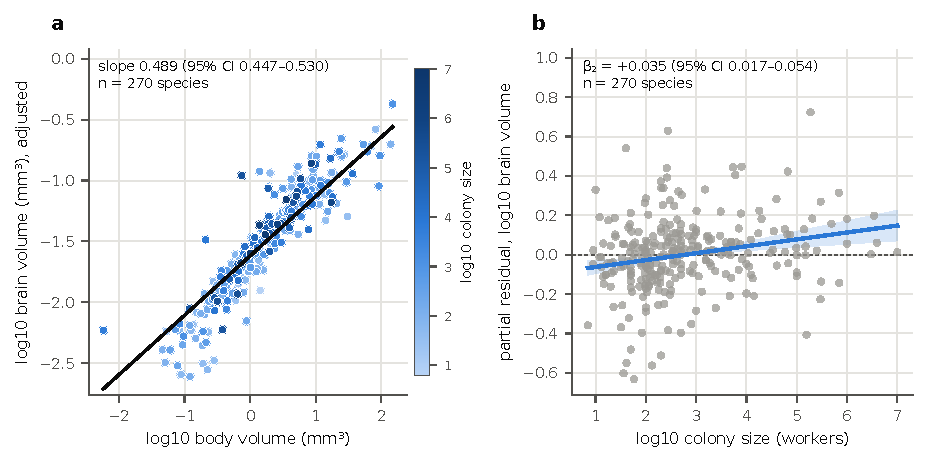
\includegraphics[width=\textwidth]{figures/fig2_allometry_colony.pdf}
\caption[Brain--body allometry and the colony-size effect]{\textbf{Brain--body allometry and the colony-size effect.}
\textbf{(a)}~Species-mean $\lten$ brain volume against $\lten$ body volume for $270$ species. Brain volume is adjusted
for stain and scan step with the coefficients of the Haller's-rule gate model. Colour shows $\lten$ colony size. The
line has the PGLS slope ($0.489$; $\lambda = 0.69$; OLS $R^2 = 0.85$) and is drawn through the species means.
\textbf{(b)}~Partial residuals (component + residual) of $\lten$ brain volume against $\lten$ colony size from the
preregistered PGLS fit~\eqref{eq:pgls} on the MCC tree ($\lambda = 0.72$). The line shows $\beta_2 = +0.035$
($p = 0.0002$), about $8.4\%$ more brain volume per tenfold colony size; the band is its $95\%$ confidence interval.}
\label{fig:allometry}
\end{figure}

\subsection{Q2: Do workers of large-colony species have smaller brains for their body size?}\label{sec:q2}

No: in the preregistered test, relative brain volume increased with colony size. On the MCC tree, $\beta_2 = +0.035$
($95\%$ CI 0.017--0.054; Figure~\ref{fig:allometry}b), with a $90\%$ CI of 0.020--0.051, $p = 0.0002$,
$\lambda = 0.72$ and $n = 270$ species. This corresponds to about $8.4\%$ more brain volume per tenfold increase in
colony size at equal body volume, stain and scan step, and the $95\%$ CI lies entirely above zero. Over the $100$
posterior trees, the median $\beta_2$ was $+0.033$ (pooled $95\%$ interval 0.014--0.051); per-tree estimates ranged
from $0.030$ to $0.035$, and every tree gave $p < 0.05$. The measurement-error model~\eqref{eq:me} gave a posterior
mean of $+0.038$ ($95\%$ credible interval, CrI, 0.019--0.055), with $P(\beta_2 > 0) = 1.000$ and
$P(\beta_2 > 0.02) = 0.97$. This estimate did not depend on the assumed measurement error: with $m = 0.0127$ it was
$+0.038$ (0.020--0.056). Most within-species variance was real worker variation ($\sigma = 0.139$ $\lten$ units)
rather than segmentation error ($m \le 0.031$). An MCMCglmm cross-check gave $+0.038$ (0.020--0.056). The
preregistered outcome is therefore support for H2 (robust); H1, smaller brains in larger colonies, is not supported.

All preregistered checks except R3 gave the same outcome, support for H2, with $\beta_2$ from $+0.024$ to $+0.042$
(Figure~\ref{fig:forest}; Table~\ref{tab:robustness}):
\begin{center}
\small
\begin{tabular}{@{}>{\raggedright\arraybackslash}p{0.33\linewidth}>{\raggedright\arraybackslash}p{0.27\linewidth}%
>{\raggedright\arraybackslash}p{0.32\linewidth}@{}}
\toprule
Check & $\beta_2$ ($95\%$ interval) & Note \\
\midrule
R1, FBD posterior trees & $+0.032$ (0.014--0.051) & on both $6$ and $200$ trees \\
R2, Borowiec tree & median $+0.029$ (pooled 0.001--0.058) & $117$ genera; 2.5--97.5\% of resamples 0.017--0.040 \\
R4, leaving out one subfamily & $+0.024$ to $+0.042$ & without Formicinae / without Myrmicinae \\
R8, without supercolonial species and social parasites & $+0.040$ (0.020--0.061) & $n = 251$ \\
R9, R10, alternative colony-size measures & $+0.027$ to $+0.041$ & \\
R12, $\lambda = 1$ & $+0.040$ & \\
R14, OLS without phylogeny & $+0.027$ (0.009--0.044) & \\
R3, owner-measured soft tissue & $+0.006$ ($-0.013$ to $0.024$) & $p = 0.56$; $n = 154$; undecided \\
\bottomrule
\end{tabular}
\end{center}
Of the $100$ R2 resamples, $77$ supported H2 and $23$ were undecided, and none gave a negative estimate. The wider
interval comes from reducing $n$ to ${\sim}117$ genera rather than from the tree: the same one-species-per-genus draws
on the Economo tree gave $+0.031$ (pooled 0.002--0.061; Table~\ref{tab:S4}). The exception was R3: with owner-measured
soft tissue as the size measure, the outcome was undecided.

\begin{figure}[tbp]
\centering
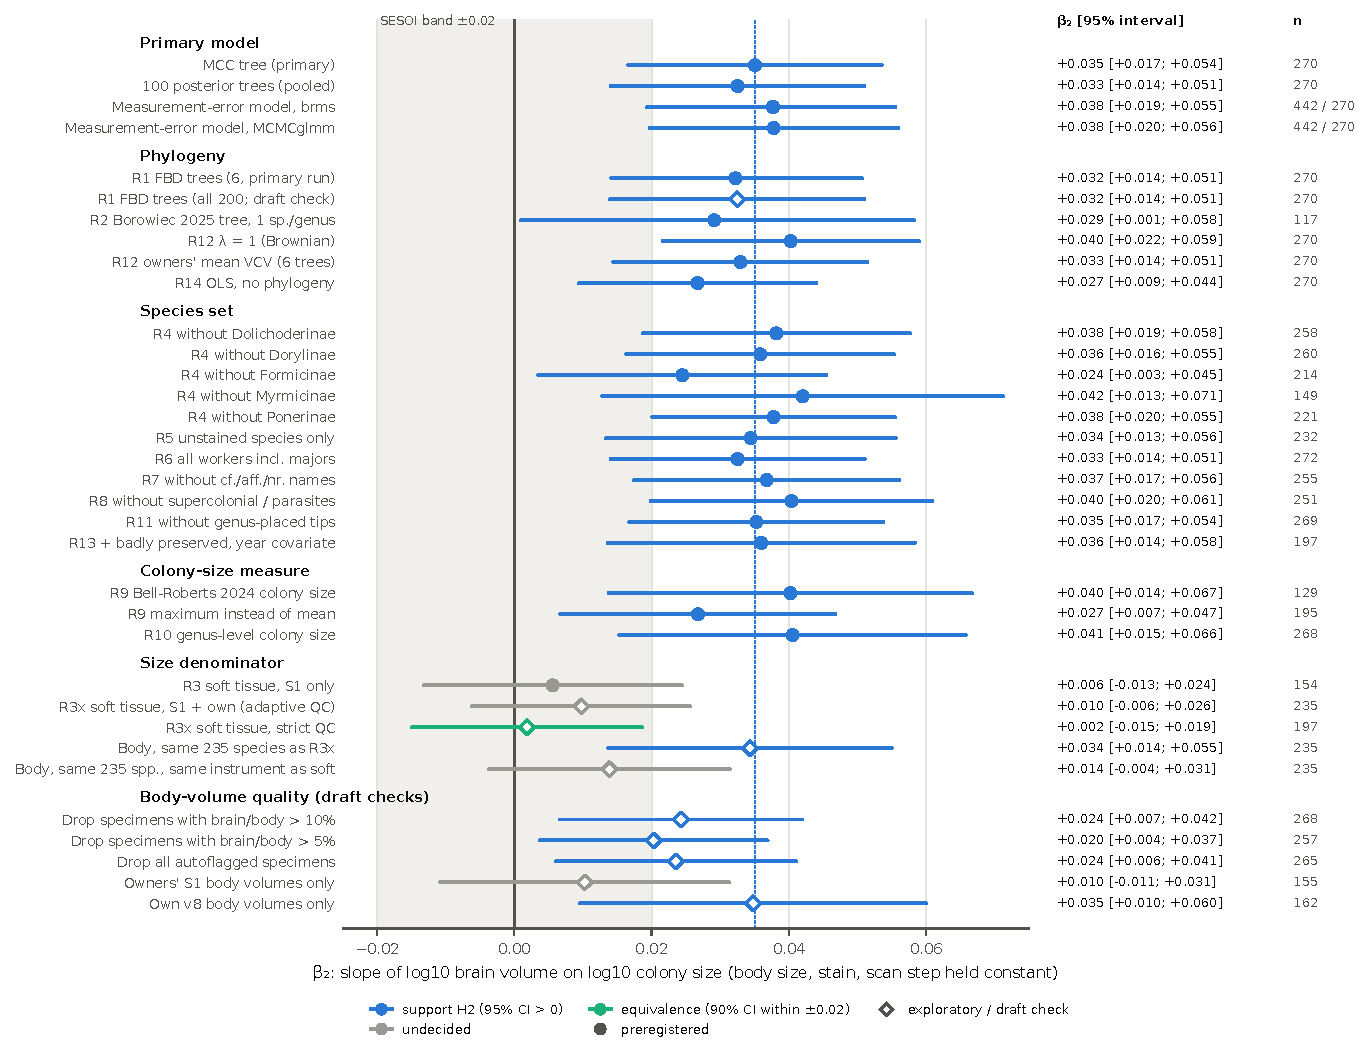
\includegraphics[width=\textwidth]{figures/fig3_forest_beta2.pdf}
\caption[$\beta_2$ across the primary analysis and all robustness checks]{\textbf{$\boldsymbol{\beta_2}$ across the
primary analysis and all robustness checks.} Points: estimates (for tree sets and resamples, medians). Lines: $95\%$
intervals (pooled intervals for tree sets and resamples; credible intervals for the measurement-error models). Grey
band: preregistered SESOI ($\pm 0.02$). Dotted line: primary estimate. Colour gives the preregistered outcome label.
Filled circles are preregistered analyses; open diamonds are exploratory analyses and post hoc checks. $n$ is the number
of species, or specimens/species for the measurement-error models.}
\label{fig:forest}
\end{figure}

\subsection{Q3: Does the estimate depend on how body size is measured?}\label{sec:q3}

Yes: in the exploratory analyses, the estimate stayed near zero with soft tissue, and the gap to the body-volume
estimate came mostly from the body-volume source rather than from thinner cuticle. Our measurements, made with the
owners' program, raised soft-tissue coverage from $154$ to $235$ of the $270$ primary species. With soft tissue as the
size measure, $\beta_2$ stayed near zero under both QC rules (Figure~\ref{fig:denominators}a; Table~\ref{tab:S6}):
\begin{center}
\small
\begin{tabular}{@{}lllll@{}}
\toprule
Rule (species) & $\beta_2$ & $95\%$ CI & $90\%$ CI & Outcome \\
\midrule
Adaptive ($235$) & $+0.010$ & $-0.006$ to $0.026$ & $-0.004$ to $0.023$ & undecided \\
Adaptive, $100$ posterior trees & median $+0.010$ & $-0.006$ to $0.026$ & n/a & no tree $p < 0.05$ \\
Strict ($197$) & $+0.002$ & $-0.015$ to $0.019$ & $-0.012$ to $0.016$ & equivalence (H0) \\
\bottomrule
\end{tabular}
\end{center}
In all soft-tissue fits, $\lambda$ was estimated at its lower bound ($\approx 0$). On the same species, the
primary-table body volume gave $+0.034$ (0.014--0.055; adaptive set) and $+0.027$ (0.007--0.047; strict set).

\paragraph{Like-for-like decomposition.} The gap between body and soft-tissue denominators could reflect thinner
cuticle in large-colony species~\citep{matte2025}. It could also reflect differences between the sources of body
volume: our body masks versus owner-measured volumes or the owners' program. The like-for-like decomposition separates
the two (Figure~\ref{fig:denominators}a; Table~\ref{tab:S6}). When body and soft tissue come from the same instrument
and the same specimens, the two denominators give similar estimates:
\begin{center}
\small
\begin{tabular}{@{}lll@{}}
\toprule
Species set & Body & Soft tissue \\
\midrule
$235$ species & $+0.014$ ($-0.004$ to $0.031$) & $+0.010$ \\
$154$ species with owner-measured soft tissue & $+0.012$ ($-0.007$ to $0.030$) & $+0.006$ \\
\bottomrule
\end{tabular}
\end{center}
The cuticle contribution is therefore about $+0.004$ to $+0.006$, and the preregistration had anticipated a bias of
about $+0.005$ from using body rather than soft tissue. The like-for-like body estimates are 0.008--0.020 below the
primary-table body estimates on the same species ($+0.020$ and $+0.034$). This result did not depend on $\lambda$: with
$\lambda$ fixed at $0$ or at $1$ for both denominators, the like-for-like body and soft-tissue estimates differed by at
most $0.006$ (Table~\ref{tab:S6}). For the $235$ species, these estimates were $+0.014$ versus $+0.010$ at
$\lambda = 0$ and $+0.016$ versus $+0.015$ at $\lambda = 1$. The gap between primary-table body and soft tissue also
persisted at matched $\lambda$ (Table~\ref{tab:S6}).

\paragraph{Thinner cuticle in large colonies.} Cuticle volume as a fraction of body volume declined with colony size
(Figure~\ref{fig:denominators}b), which reproduces the pattern of \citet{matte2025} in our species set. The correlation
$r(\lten\text{colony}, \lten\text{soft/body})$ was $+0.26$ for the $235$ species and $+0.39$ for the $154$ species
with owner-measured soft tissue.

\begin{figure}[tbp]
\centering
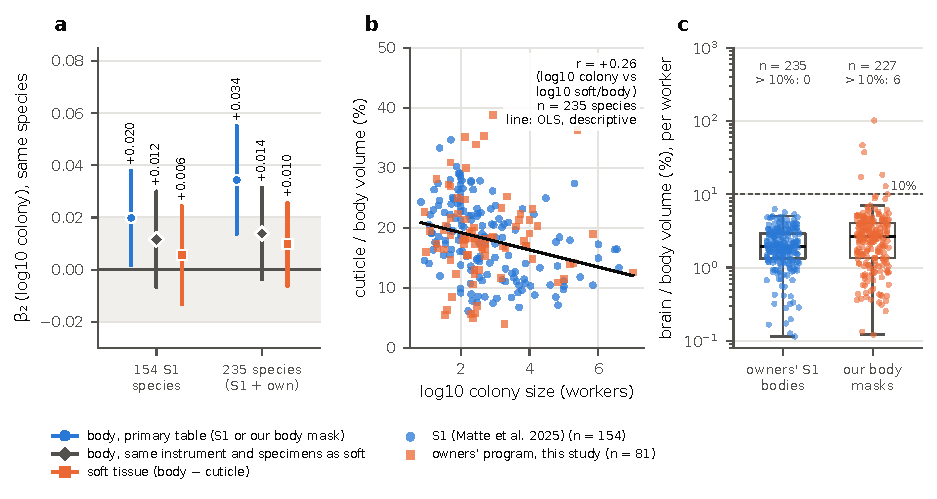
\includegraphics[width=\textwidth]{figures/fig4_denominators_cuticle.pdf}
\caption[Size denominators, cuticle and body-volume quality]{\textbf{Size denominators, cuticle and body-volume
quality.} \textbf{(a)}~$\beta_2$ for the same species with three size measures: body volume from the primary table
(S1 or our body mask); body volume from the same instrument and specimens as the soft-tissue measure (S1 or the owners'
program); soft tissue. Shown for the $154$ species with S1 soft tissue and for the $235$ species of the extended set.
Lines are $95\%$ CIs; the grey band is the SESOI.
\textbf{(b)}~Cuticle volume as a percentage of body volume (same specimens) against $\lten$ colony size. Colour gives
the source: S1 or our run of the owners' program. The line is OLS and descriptive only.
\textbf{(c)}~Brain/body volume ratio of main-analysis workers by body-volume source (log scale). The dashed line marks
the preregistered plausibility limit of $10\%$.
In all legends, S1 denotes owner-measured volumes (Dataset S1 of \citealp{matte2025}); our body masks are described in
Section~\ref{sec:body}.}
\label{fig:denominators}
\end{figure}

\paragraph{Body-volume quality.} Brain/body ratios point to errors in a small number of body volumes from our
masks (Figure~\ref{fig:denominators}c; Table~\ref{tab:S9}). With owner-measured bodies, the median brain/body ratio was
$1.95\%$, and no worker was above $10\%$. For bodies from our masks, the median was $2.64\%$, and $6$ workers were above $10\%$,
with a maximum of $102\%$, which is physically impossible; $28$ workers were above $5\%$. Refits of the primary
model~\eqref{eq:pgls} (Table~\ref{tab:robustness}, ``post hoc check'' rows) gave:
\begin{center}
\small
\begin{tabular}{@{}llll@{}}
\toprule
Change to the primary data & $\beta_2$ & $95\%$ CI & Species \\
\midrule
Remove the $6$ workers with brain/body $> 10\%$ & $+0.024$ & 0.007--0.042 & $268$ \\
Remove workers with brain/body $> 5\%$ & $+0.020$ & 0.004--0.037 & $257$ \\
Owner-measured (S1) bodies only & $+0.010$ & $-0.011$ to $0.031$ & $155$ \\
Bodies from our masks only & $+0.035$ & 0.010--0.060 & $162$ \\
\bottomrule
\end{tabular}
\end{center}
The first two refits still support H2, whereas the fit with owner-measured bodies only is undecided. The brain--body
slope was steeper with owner-measured bodies ($0.645$) than in the primary fit ($0.473$), which is consistent with
measurement error in our body masks attenuating the size slope. Because colony size correlates weakly with body size
($r = 0.13$), part of the unexplained size signal can then load onto $\beta_2$. The six workers with brain/body
$> 10\%$ belong to five species, among them two large-colony species (\emph{Linepithema humile}, \emph{Pheidole
bicarinata}; Table~\ref{tab:S9}).

\paragraph{Across all analyses.} Every estimate in Table~\ref{tab:robustness} was positive (minimum $+0.002$), and
every lower $95\%$ bound was above $-0.02$ (lowest $-0.015$). Negative effects of the size the preregistration deemed
relevant are therefore excluded throughout. Only in the $\lambda = 1$ sensitivity fits of the $81$ own-measured species
(Table~\ref{tab:S6}) were estimates slightly negative ($-0.003$), with wide intervals.

\section{Discussion}\label{sec:discussion}

\paragraph{Main result.} Across $270$ ant species, workers of species with larger colonies do not have smaller brains
for their size. The distributed-cognition prediction of brain downsizing (H1) is not supported by any analysis. This
holds for the preregistered test, $14$ robustness checks, two phylogenies, a model of measurement error, two
soft-tissue denominators and several body-quality filters. Every interval in Table~\ref{tab:robustness} excludes a
reduction as large as the preregistered SESOI (about $4.5\%$ brain volume per tenfold colony size). For a comparative
test across $123$ genera, this is strong evidence against a general economy on neural tissue in large societies.

\paragraph{A modest positive association.} The positive association (H2) is real by the preregistered criterion, but
modest and sensitive to the body measure. The primary estimate ($+0.035$, about $8\%$ per tenfold colony size) passed
every preregistered robustness check except the soft-tissue denominator. Exploratory analyses that use the most
accurate size measures put the effect at $+0.006$ to $+0.014$, with intervals that include zero. These measures are
the owners' body volumes, body and soft tissue from the same instrument, and soft tissue. Part of the primary estimate
is attributable to errors in a minority of our own body masks. We therefore read the data as showing that brain
investment is maintained in large-colony species, possibly with a small increase, and we do not read them as strong
support for the social-brain hypothesis. Remeasuring all body volumes with the owners' program
would resolve how large the positive effect is.

\paragraph{Cheaper workers, but not cheaper brains.} \citet{matte2025} showed that workers of large-colony species
invest less in cuticle, and our data reproduce that pattern. We find that this economy does not extend to the brain:
relative to soft tissue, brain volume does not decline with colony size, and possibly increases slightly. Thinner
cuticle accounts for only about $0.005$ of the body-denominator slope, close to the preregistered expectation. Large
societies thus economise on protective tissue but not on neural tissue.

\paragraph{Relation to earlier studies.} Our broad result is consistent with \citet{perl2026}, who found no larger
brains in \emph{Pogonomyrmex} species with larger colonies. It also agrees with studies finding no colony-size effect
on specific neuropils~\citep{godfrey2020,marty2025}. In contrast, \citet{riveros2012} found smaller relative brains in
large-colony monomorphic attines ($18$ species). Narrow clades, specific ecologies or worker polymorphism may produce
local patterns that do not generalise across the family. Distributed cognition may still act on brain composition
rather than total volume, for example on mushroom bodies~\citep{odonnell2015,kamhi2016,kamhi2019}. Whole-brain volume
cannot test that, and neuropil-level segmentation of AntScan is a natural next step.

\subsection{Limitations}\label{sec:limitations}

Our study has several limitations.
\begin{itemize}
\item \textbf{AntScan scan classes.} Voxel size (\qtyrange{1.22}{6.11}{\um}) and staining differ between specimens
and are partly confounded with body size. Both enter the model; the coefficient for the \qty{1.22}{\um} class was
$-0.138$ ($-0.244$ to $-0.031$; Table~\ref{tab:S3}), and analyses restricted to unstained species (R5) gave the same
outcome.
\item \textbf{Colony-size data.} Colony sizes are species means compiled from the literature; they are often based on
few records and vary within species. Error in the predictor tends to attenuate $\beta_2$ towards zero, which limits
precision but is unlikely to create a positive estimate. Alternative colony measures (R9, R10) gave the same outcome.
\item \textbf{Vision-agent QC instead of human review.} All inclusion decisions were made by a language-model agent; in
the final round, one agent verdict per mask. The agent-approved masks agree closely with the final ensemble, and
accuracy against human labels is high. Still, no human audit of a random sample has been done.
\item \textbf{Body volume.} Our own body masks contain a few gross errors (Section~\ref{sec:q3}). The preregistered
pipeline flagged brain/body ratios outside 0.05--10\% but did not exclude them, and this is the main reason why the
effect size is uncertain.
\item \textbf{Soft-tissue coverage.} Soft tissue is available for $235$ of $270$ species ($197$ under strict QC). The
$35$ missing species are those whose measured workers all failed QC, mostly because a bright mounting medium leaked
into the mask (\qty{6.11}{\um} scans failed in $17$ of $31$ cases).
\item \textbf{Cuticle QC rule.} The adaptive rule was written after an interim look ($+0.007$ on $28$ species) and
revised once, without looking at estimates under it. Both versions are reported, and both give estimates near zero
($+0.010$ and $+0.002$).
\item \textbf{Subsampled slices.} Our runs of the owners' program read every third slice; the effect on volumes was
below $0.1\%$ (median), with a maximum deviation of $2.2\%$ for soft tissue.
\item \textbf{Departures from the preregistered plan.} R1 originally used $6$ instead of $200$ trees (recomputed here),
R10 is an approximation, and the head-volume variant of R3 and the secondary analyses were not run.
\end{itemize}

\subsection{Conclusion}\label{sec:conclusion}

We conclude that, across $270$ ant species, workers of species with larger colonies do not have smaller brains. The
preregistered test found a positive association between colony size and relative brain volume, but its magnitude
shrinks to a small, uncertain value when the most accurate size measures are used. Negative effects of practical size
are excluded in every analysis in Table~\ref{tab:robustness}. Large ant societies economise on worker cuticle but not
on worker brains.

\needspace{10\baselineskip}
\phantomsection
\section*{Data and code availability statement}\label{sec:data}

\paragraph{Code and data.}
\begin{itemize}
\item \textbf{Code repository.} The measurement pipeline and analysis code are public at
\url{https://github.com/daglar-dragomirov/ant-twin}; every run records the exact code commit it used. The
\texttt{paper/} folder of the repository contains the preregistration, the result reports, the analysis and robustness
scripts (including those that generate every figure and table, with the selection rules and seeds of the image
figures), a storage index listing every run and file, and the manuscript source.
\item \textbf{Stored data.} The frozen brain table, all masks, vision-agent verdicts and QC images, model weights, run
logs and the outputs of the primary and robustness analyses are kept in object storage. They are available from the
corresponding author on request until the archive described below is released.
\item \textbf{Preregistration.} Frozen on 15 November 2026 (13:07 UTC+3) as tag \texttt{ant-twin-prereg-v1.0}
(commit \texttt{c01e2ee}; freeze commit \texttt{3b1e350}) in the author's project repository, before any model containing
colony size was fitted to real brain volumes. The frozen files are reproduced unchanged in the \texttt{paper/} folder of
the public repository (SHA-256 of the frozen plan, version 1.0: \texttt{212bc991\ldots{}5230}; of the initial version
0.1: \texttt{94689629\ldots{}2c2e}); the history of the project repository is available to editors and reviewers on
request.
\end{itemize}

\paragraph{Planned archive.} A release with a DOI (Zenodo) will contain the brain table, species tables, masks, QC
verdicts and the analysis code.

\paragraph{Third-party data.}
\begin{itemize}[nosep]
\item AntScan scans: CC BY 4.0~\citep{katzke2026}.
\item \citet{matte2025} data and segmentation program: Zenodo 15546461, CC BY 4.0.
\item \citet{economo2018} trees: Dryad doi:\nolinkurl{10.5061/dryad.g579t7k}, CC0.
\item \citet{borowiec2025} trees: Zenodo 14338504, CC BY 4.0.
\item \citet{toulkeridou2023} labels: Dryad doi:\nolinkurl{10.5061/dryad.qz612jmgv}, CC0.
\item \citet{bellroberts2024}: supplementary tables.
\end{itemize}

\section*{AI use statement}

Large-language-model assistants (Claude, Anthropic) were used in this project as research tools, in the same way as
other research software, with every step directed by the author. They helped design and write the measurement and
analysis code (brain localisation, segmentation training and inference, the body- and cuticle-measurement wrappers,
the PGLS and robustness scripts) under the author's direction; ran and monitored the cloud computations; drafted the
preregistration and the analysis plan; summarised and interpreted results; and drafted, edited and translated text,
which the author reviewed. They were also used for literature search, figure preparation and reference formatting.

In one place AI is part of the measurement protocol rather than an assistant: mask quality control was performed by
vision-capable agents (Claude Opus 5.5) following a fixed written protocol (verdict ``good'' means that the box is on
the head and the brain lies entirely inside it), with a second review of disputed masks. All verdicts and QC images
are archived (Section~\ref{sec:brain}; Appendix~\ref{app:dev}, deviation~\ref{dev:qc}; Data and code availability
statement).

No claim of the paper rests on the assistants alone. Verification relied on checks that do not depend on the
assistants' judgement: segmentation accuracy was measured against human expert labels of held-out species
(\citealp{toulkeridou2023}; Dice 0.962--0.973); body and soft-tissue volumes were validated against the owners'
published measurements of the same specimens~\citep{matte2025}; the statistical model was cross-checked against
independent R implementations (\texttt{nlme}, \texttt{phylolm}; differences below $10^{-6}$) and by synthetic recovery
on the real tree; the analysis plan was frozen in a timestamped commit before unblinding; every reported number is
regenerated from frozen records by the released scripts; and every reference was checked against Crossref or
DataCite. The assistants supplied no measurements: all volumes are computed by deterministic code from the AntScan
scans, and colony sizes and phylogenies come from published sources. The author takes full responsibility for the
content of this paper, including any text, claims or code produced with the aid of these tools.

\section*{Software}

Brain segmentation used nnU-Net v2 \citep{isensee2021}. Statistical analyses used R~4.6.2 \citep{rcore2026} with
nlme~3.1-171 \citep{pinheiro2026nlme}, phylolm~2.6.5 \citep{ho2014}, ape \citep{paradis2019}, brms \citep{burkner2017}
with Stan through cmdstanr \citep{carpenter2017}, and MCMCglmm \citep{hadfield2010}; the pipeline was written in
Python~3.13.

\section*{Acknowledgements}

I thank the AntScan team and the authors of \citet{toulkeridou2023}, \citet{matte2025}, \citet{economo2018},
\citet{borowiec2025} and \citet{bellroberts2024} for making their data and code openly available. This work received
no specific funding.

\section*{Author contributions statement}

D.D. is the sole author: he designed the study, wrote the preregistration and the code, performed the analyses and
wrote the paper.

\section*{Competing interests statement}

The author declares no competing interests.

\bibliographystyle{plainnat}
\bibliography{refs}

\appendix
\section{Deviations from the preregistration}\label{app:dev}

The protocol, including its deviations, is described here.

\paragraph{Declared at the freeze (prereg v1.0).}
\begin{enumerate}[series=deviations]
\item\label{dev:seg} Segmentation uses the seg v3 ensemble (Toulkeridou labels + agent-approved AntScan brains) instead
of a model trained on Toulkeridou labels only.
\item\label{dev:qc} Mask QC is done by vision agents instead of human review.
\item\label{dev:body} Body volume uses v8 instead of v6. The v6 slice spacing was wrong for compressed stacks; the
median ratio to the owner-measured volumes (S1) changed from $1.15$ to $1.04$.
\item\label{dev:reg} Registration is a timestamped GitHub commit and tag instead of OSF. The repository is private
until the preprint is posted.
\item\label{dev:metime} The measurement-error model was run after the primary test.
\end{enumerate}

\paragraph{After unblinding.}
\begin{enumerate}[resume=deviations]
\item\label{dev:melength} \textbf{Measurement-error model, run length.} It used $4 \times 4000$ iterations instead of
$4 \times 2000$. With $2000$ iterations, one variance component had bulk ESS $372$ ($< 400$). The 2000-iteration
estimate is $+0.0375$ (0.0193--0.0554).
\item\label{dev:mem} \textbf{Measurement-error model, $\boldsymbol{m}$.} $m$ is the held-out error only. The
per-specimen between-fold spread named in the preregistration was not recorded by the ensemble.
\item\label{dev:backend} \textbf{Measurement-error model, backend.} cmdstanr was used instead of rstan (compilation
failure); model and priors unchanged.
\item\label{dev:r2pool} \textbf{R2 species pool.} $272$ species ($270 + 2$ species placed only in the Borowiec tree);
the 270-species version is reported alongside (Table~\ref{tab:S4}).
\item\label{dev:r8} \textbf{R8 flags.} Only Bell-Roberts Table 21 was used, as preregistered; unlisted species count as
unflagged.
\item\label{dev:r1} \textbf{R1 tree count.} R1 used $6$ FBD trees ($3$ crown + $3$ stem), because the analysis
configuration capped tree sets at $6$. The preregistration names $200$. The owners'-method variant of R12 averaged the
same $6$ trees. Both were recomputed on all $200$ trees for this draft; the results are unchanged
(Table~\ref{tab:robustness}).
\item\label{dev:r10} \textbf{R10.} Implemented as an approximation: genus medians of the species-level S3 means in our
species table. The planned extension to ${\sim}746$ species without species-level colony size was not built.
\item\label{dev:notrun} \textbf{Not run.} The head-volume variant of R3 (no head masks were produced), and the three
secondary analyses of prereg Section~9 (number of worker castes, number of queens, path analysis).
\item\label{dev:r3x} \textbf{R3 extension.} Measurement protocol and QC rule were specified after unblinding. The QC
rule was fixed before the final fits and revised once, on segmentation diagnostics. An interim estimate on $28$ added
species ($+0.007$) had been seen before the rule was written. Both rule versions are reported.
\item\label{dev:brain} \textbf{Brain definition.} The preregistration's TODO to record the exact Toulkeridou label
definition is still open (Section~\ref{sec:brain}).
\end{enumerate}

ESS is the effective sample size of the sampler.

\section{Implementation details}\label{app:impl}

\paragraph{Scan stacks.} Low-resolution copies were cached for $811$ stacks. The true number of slices of every
full-resolution stack was read from the first image file directory of the tagged image file format (TIFF); a
size-based estimate had been wrong for $551$ compressed stacks.

\paragraph{Frozen brain table.} The table was frozen before unblinding (SHA-256
\path{df1902432f4680b295c1e68cc68804c6d42a71a445d0dbd2003f90bbaf646ead}).

\paragraph{Registration.} The analysis plan and outcome rules were preregistered as version 0.1
(13 November 2026). The plan was frozen, with the deviations listed in Appendix~\ref{app:dev}, in commit
\texttt{3b1e350} and tag \texttt{ant-twin-prereg-v1.0} (commit \texttt{c01e2ee}, wording fix) on 15 November 2026.

\paragraph{R2 details.}
\begin{itemize}[nosep]
\item The Borowiec tree has one exemplar per genus. Each of the $100$ resamples (seed 2025) attaches one random species
per genus to that genus' tip.
\item Main dating scheme: root prior 129--158~Ma with independent rates. The other three schemes are reported as
sensitivity.
\item The species pool was all $272$ species with brain, body and colony size; two of them are absent from the Economo
tree. $117$ of $125$ genera matched.
\end{itemize}

\paragraph{R8 details.}
\begin{itemize}[nosep]
\item $19$ of the $270$ primary species were flagged: $14$ supercolonial, $4$ social parasites, $1$ both.
\item Species outside the Bell-Roberts set were treated as unflagged.
\end{itemize}

\paragraph{Measurement-error model} (specimen level; brms 2.23 with CmdStan 2.37). The brms formula is
\begin{small}
\begin{verbatim}
log10_brain | se(m, sigma = TRUE) ~ log10_body + log10_colony + iodine
    + step1.22 + step6.11 + (1 | gr(phylo, cov = A)) + (1 | species)
\end{verbatim}
\end{small}
In model notation, for specimen $i$ of species $s(i)$, with $y_i$ its $\lten$ brain volume,
\begin{equation}\label{eq:me}
\begin{gathered}
y_i \sim \Normal\bigl(\mu_i,\; \sigma^2 + m^2\bigr), \qquad
\mu_i = \vx_i^{\top}\boldsymbol{\beta} + a_{s(i)} + u_{s(i)},\\
\mathbf{a} \sim \Normal\bigl(\mathbf{0},\, \sigma_{\mathrm{phylo}}^2\Amat\bigr), \qquad
u_s \sim \Normal\bigl(0,\, \sigma_{\mathrm{species}}^2\bigr),
\end{gathered}
\end{equation}
where $\vx_i$ holds the intercept and the covariates of model~\eqref{eq:pgls} ($\lten$ body volume, $\lten$ colony
size, iodine, step 1.22, step 6.11), $m$ is the known measurement SD, $\sigma$ the residual (worker-level) SD, and
$\mathbf{a}$ and $u$ are the phylogenetic and species-level random intercepts.
\begin{itemize}[nosep]
\item Data: $442$ specimens of the $270$ species. $\Amat$ is the MCC correlation matrix.
\item Known measurement SD: $m = \lten(1 + 0.05/0.6745) = 0.0311$, from the held-out AntScan volume error.
Sensitivity: $m = 0.0127$, from the human-labelled folds.
\item Priors as preregistered: $b \sim \Normal(0, 0.5)$, intercept $\sim t_3(0, 2.5)$, SDs $\sim$ half-$t_3(0, 0.5)$.
\item Sampling: $4$ chains $\times$ $4000$ iterations (Appendix~\ref{app:dev}, item~\ref{dev:melength}).
\item An MCMCglmm fit ($4 \times 260{,}000$ iterations) served as a cross-check.
\end{itemize}

\clearpage
\section{Supplementary figures}\label{app:suppfig}

\setcounter{figure}{0}
\renewcommand{\thefigure}{S\arabic{figure}}
\renewcommand{\theHfigure}{S\arabic{figure}}

Supplementary Figures~\ref{fig:tk}--\ref{fig:qcrej} show cases chosen by fixed rules with a fixed seed, not the
best-looking ones. The rules are stated in each legend; the inputs are listed in the code repository's storage
index.

\begin{figure}[htbp]
\centering
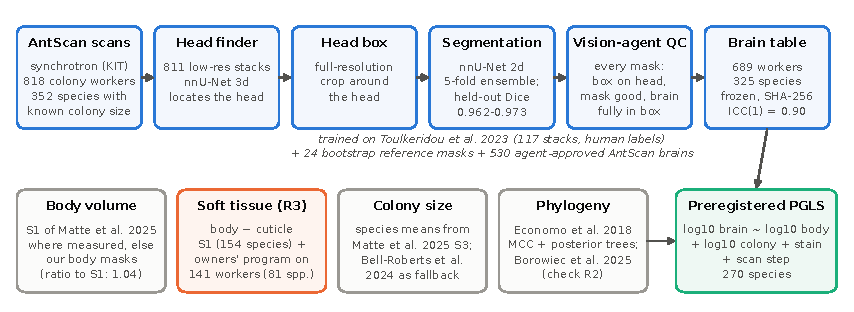
\includegraphics[width=0.9\textwidth]{figures/figS1_pipeline_schematic.pdf}
\caption[Measurement and analysis pipeline (schematic)]{\textbf{Measurement and analysis pipeline (schematic).}
AntScan synchrotron scans of colony workers pass through low-resolution brain localisation, a full-resolution head
box, the segmentation ensemble (nnU-Net 2d, 5 folds), vision-agent QC and the frozen brain table. Body volume, soft
tissue, colony size and the phylogeny enter the preregistered PGLS model~\eqref{eq:pgls}. Figure~\ref{fig:scan} shows
the same steps on real scans.}
\label{fig:schematic}
\end{figure}

\begin{figure}[htbp]
\centering
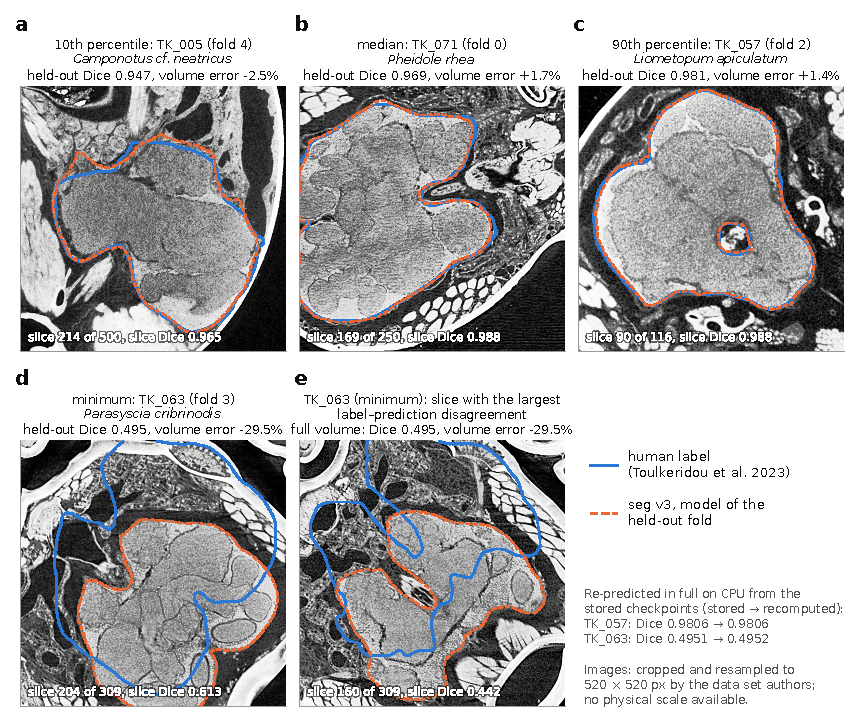
\includegraphics[width=0.86\textwidth]{figures/figS2_tk_heldout.pdf}
\caption[Segmentation model against human labels on held-out Toulkeridou cases]{\textbf{Segmentation model against
human labels on held-out Toulkeridou cases.} Four of the $117$ human-labelled stacks of \citet{toulkeridou2023} that were held out in
cross-validation. \emph{Selection rule:} the cases nearest the 10th, 50th and 90th percentile of per-case held-out
Dice (a--c) and the case with the lowest Dice (d--f). Each case was predicted by the segmentation model of the fold
whose validation set contains it; folds were split by species, so the species was not in training. Blue: human
label; orange, dashed: segmentation model of the held-out fold.
\textbf{(a--d)}~The slice with the largest labelled area. Titles give the held-out Dice and volume error of the full
volume; tiles give the Dice of the shown slice.
\textbf{(e)}~For the lowest case, the slice with the largest label--prediction disagreement.
\textbf{(f)}~The same slice with the human label moved by the rigid offset described below.
In the lowest case, the label in the deposited training archive is offset from its image by about
$115 \times 27$~pixels on every slice; moved back by this rigid shift, it outlines the brain (panel f; full-volume
Dice $0.812$ instead of $0.495$). The shifted label is still about $1.4$ times larger than the predicted brain, so the
deposited label was probably drawn on a differently cropped version of the image. A check of all $117$ held-out
reference labels (rigid-offset rule fixed before the check: shift $\geq 5$~px, Dice gain $\geq 0.10$, consistent
across slices) flagged only this stack. We kept it in Figure~\ref{fig:scan}d--e and Table~\ref{tab:S2}; without it
the median Dice is unchanged. Across the $117$ cases the median Dice was $0.969$, and $3$ cases were below $0.90$.
The dataset authors cropped and resampled the images to $520 \times 520$ pixels per slice, so no physical scale is
given.}
\label{fig:tk}
\end{figure}

\begin{figure}[htbp]
\centering
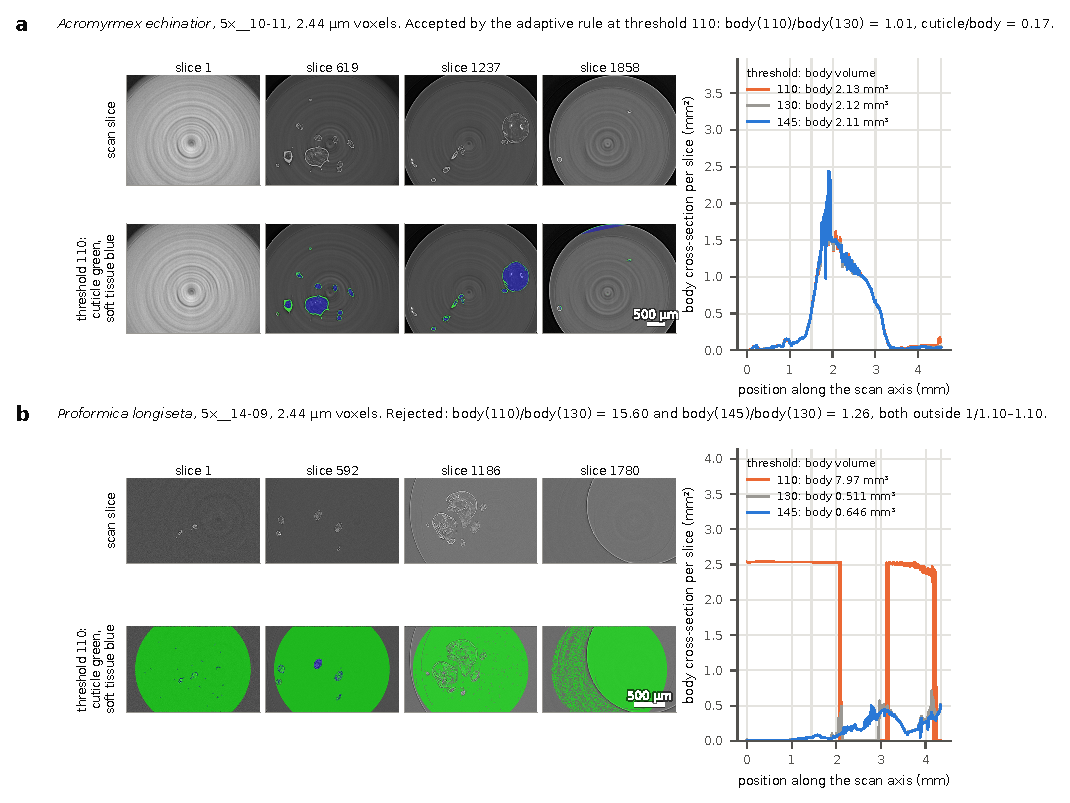
\includegraphics[width=\textwidth]{figures/figS3_cuticle_qc.pdf}
\caption[Body and cuticle segmentation by the owners' program, and the QC rule]{\textbf{Body and cuticle segmentation
by the owners' program, and the QC rule.} One specimen accepted and one rejected by the adaptive rule
(Section~\ref{sec:body}). \emph{Selection rule:} drawn at random (seed 20261116) from the $92$ specimens accepted at
threshold $110$ and from the $21$ specimens rejected with $\body{110}/\body{130} > 1.10$, the signature of a bright
mounting medium entering the mask. These $21$ are among the $37$ specimens for which neither threshold gave a stable
body volume; $7$ further specimens failed the cuticle/body limits. Left: the QC sheet written by our run of the
owners' program, with its tiles rearranged. The top row shows four evenly spaced slices of the processed range, and
the bottom row the segmentation at threshold $110$ (cuticle green, soft tissue blue). Right: body cross-section of
every sampled slice (every third slice) at thresholds $110$, $130$ and $145$, with the specimen's body volume at each
threshold; grey lines mark the slices shown on the left.
\textbf{(a)}~Accepted: the three thresholds give the same body ($\body{110}/\body{130} = 1.01$).
\textbf{(b)}~Rejected: at threshold $110$ the mounting medium fills the vial over long stretches of the stack, so
$\body{110}$ is $15.6$ times $\body{130}$; threshold $145$ also differs from $130$ by more than $10\%$.}
\label{fig:cuticle}
\end{figure}

\begin{figure}[htbp]
\centering
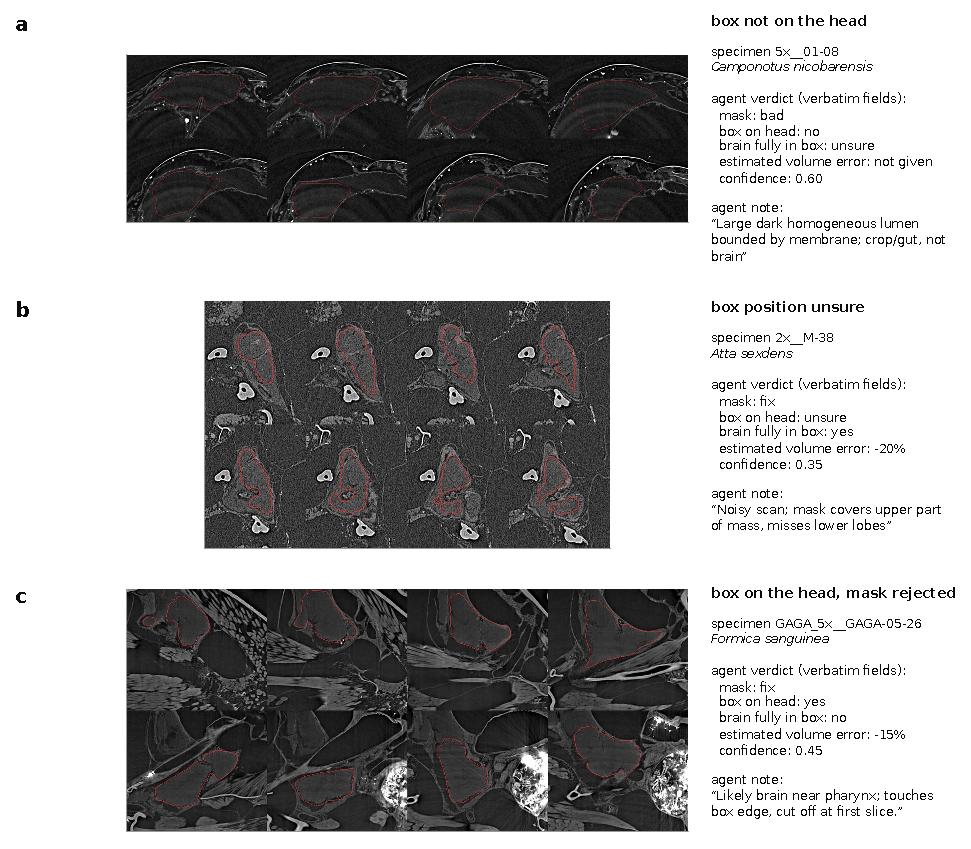
\includegraphics[width=0.92\textwidth]{figures/figS4_qc_rejections.pdf}
\caption[Masks rejected by the vision-agent QC]{\textbf{Masks rejected by the vision-agent QC.} Three masks from the
final QC round on masks of the segmentation ensemble in boxes from the final head finder: $268$ masks were reviewed, $124$ accepted and
$144$ rejected. The rejected masks fall into three categories by the agent's box verdict: box not on the head ($62$),
box position unsure ($45$) and box on the head but mask not good or brain not fully in the box ($37$).
\emph{Selection rule:} within each category, one mask was drawn at random (seed 20261116) among specimens absent from
the frozen table and with a non-empty mask ($20$, $25$ and $28$ eligible). Left: the contact sheet exactly as the
agent reviewed it: eight slices through the head box with the mask outline in red. Right: the verdict fields and the
agent's note, verbatim.
\textbf{(a)}~The agent judged the masked structure to be the crop or gut, not the brain.
\textbf{(b)}~The agent could not decide whether the box was on the head, and judged the mask incomplete.
\textbf{(c)}~The agent judged the box to be on the head but the brain to be cut off by a box face.}
\label{fig:qcrej}
\end{figure}

\clearpage
\section{Supplementary tables}\label{app:supptab}

\setcounter{table}{0}
\renewcommand{\thetable}{S\arabic{table}}
\renewcommand{\theHtable}{S\arabic{table}}

Supplementary Tables~\ref{tab:S1}--\ref{tab:S10} are generated by the released analysis scripts from the stored
result files (Data and code availability statement). Outcome labels, interval conventions and the meaning of ``post hoc
check'' are as in Table~\ref{tab:robustness}. S1 denotes owner-measured volumes (Dataset S1 of \citealp{matte2025});
``own'' and ``our body masks'' refer to the body masks of Section~\ref{sec:body}.

\begin{table}[htbp]
\centering
\caption[Sample funnel]{\textbf{Sample funnel.}}
\label{tab:S1}
\footnotesize
\begin{tabular}{@{}>{\raggedright\arraybackslash}p{10.5cm}l@{}}
\toprule
Step & Count \\
\midrule
Target set: colony workers of species with colony size & 818 specimens / 352 species \\
Workers with an agent-approved brain mask (frozen table) & 689 specimens / 325 species \\
Excluded for damage (head/anterior truncation etc.) & 12 \\
Brain OK & 677 \\
Excluded major / media / intercaste (main analysis) & 49 \\
Main-analysis workers & 628 \\
Main-analysis workers with body volume & 462 (S1 235, our body masks 227) \\
Species with QC brain & 322 \\
Species with QC brain and body & 272 \\
Species with brain, body, colony size, in the Economo tree (primary n) & 270 \\
\quad of which unstained & 232 \\
\bottomrule
\end{tabular}
\end{table}

\begin{table}[htbp]
\centering
\caption[Segmentation accuracy on held-out folds (species-level folds within each source)]{\textbf{Segmentation accuracy of our segmentation model on held-out folds (species-level folds within each source).}}
\label{tab:S2}
\footnotesize
\begin{tabular}{@{}cllrr@{}}
\toprule
Fold & Reference & $n$ & Dice (median) & $|$volume error$|$, median (\%) \\
\midrule
0 & Toulkeridou 2023, human labels & 22 & 0.9709 & 0.97 \\
0 & AntScan, bootstrap reference masks & 7 & 0.9267 & 4.89 \\
0 & AntScan, agent-approved reference masks & 103 & 0.9833 & 0.99 \\
\addlinespace
1 & Toulkeridou 2023, human labels & 25 & 0.9711 & 2.01 \\
1 & AntScan, bootstrap reference masks & 5 & 0.9194 & 8.88 \\
1 & AntScan, agent-approved reference masks & 107 & 0.9845 & 0.97 \\
\addlinespace
2 & Toulkeridou 2023, human labels & 22 & 0.9618 & 2.2 \\
2 & AntScan, bootstrap reference masks & 5 & 0.9555 & 5.0 \\
2 & AntScan, agent-approved reference masks & 113 & 0.983 & 1.11 \\
\addlinespace
3 & Toulkeridou 2023, human labels & 24 & 0.9728 & 1.53 \\
3 & AntScan, bootstrap reference masks & 3 & 0.9174 & 2.96 \\
3 & AntScan, agent-approved reference masks & 102 & 0.9847 & 1.05 \\
\addlinespace
4 & Toulkeridou 2023, human labels & 24 & 0.9657 & 2.56 \\
4 & AntScan, bootstrap reference masks & 4 & 0.9365 & 5.46 \\
4 & AntScan, agent-approved reference masks & 105 & 0.9817 & 1.21 \\
\bottomrule
\end{tabular}
\end{table}

\begin{table}[htbp]
\centering
\caption[Coefficients of the primary model and the Haller's-rule gate]{\textbf{Coefficients of the primary model and the Haller's-rule gate.}}
\label{tab:S3}
\footnotesize
\begin{tabular}{@{}lrrrrrr@{}}
\toprule
Term & Estimate & SE & $t$ & $p$ & CI low & CI high \\
\midrule
\multicolumn{7}{@{}l}{\emph{Primary (MCC, $\lambda = 0.717$, $n = 270$)}} \\
\texttt{(Intercept)} & $-1.78137$ & 0.07852 & $-22.68678$ & 0.0 & $-1.93598$ & $-1.62677$ \\
\texttt{log10\_body} & 0.47333 & 0.02088 & 22.6727 & 0.0 & 0.43223 & 0.51444 \\
\texttt{log10\_colony\_any} & 0.03506 & 0.00938 & 3.7362 & 0.00023 & 0.01658 & 0.05354 \\
\texttt{stainiodine} & 0.02986 & 0.02969 & 1.00564 & 0.31551 & $-0.0286$ & 0.08832 \\
\texttt{vox\_class1.22} & $-0.13766$ & 0.05404 & $-2.54726$ & 0.01142 & $-0.24407$ & $-0.03125$ \\
\texttt{vox\_class6.11} & 0.05999 & 0.036 & 1.6665 & 0.0968 & $-0.01089$ & 0.13087 \\
\addlinespace
\multicolumn{7}{@{}l}{\emph{Haller's-rule gate (no colony, $\lambda = 0.685$, $n = 270$)}} \\
\texttt{(Intercept)} & $-1.69402$ & 0.07397 & $-22.90203$ & 0.0 & $-1.83966$ & $-1.54838$ \\
\texttt{log10\_body} & 0.48851 & 0.02105 & 23.20322 & 0.0 & 0.44706 & 0.52997 \\
\texttt{stainiodine} & 0.03529 & 0.03053 & 1.15606 & 0.2487 & $-0.02482$ & 0.0954 \\
\texttt{vox\_class1.22} & $-0.14092$ & 0.0555 & $-2.53913$ & 0.01169 & $-0.2502$ & $-0.03164$ \\
\texttt{vox\_class6.11} & 0.0677 & 0.03704 & 1.82801 & 0.06867 & $-0.00522$ & 0.14062 \\
\bottomrule
\end{tabular}
\end{table}

\begin{table}[htbp]
\centering
\caption[R2: Borowiec et al. 2025 tree, all dating schemes and species sets]{\textbf{R2: \citet{borowiec2025} tree, all dating schemes and species sets.}}
\label{tab:S4}
\scriptsize
\setlength{\tabcolsep}{3pt}
\begin{tabular}{@{}>{\raggedright\arraybackslash}p{2.6cm}>{\raggedright\arraybackslash}p{2.4cm}rrrccrrr@{}}
\toprule
Tree / dating scheme & Species set & \makecell[br]{Re-\\samples} & Genera & \makecell[br]{Median\\$\beta_2$} & \makecell[bc]{2.5--97.5\%\\of resamples} & \makecell[bc]{Pooled\\$95\%$ CI} & \makecell[br]{Share\\H2} & \makecell[br]{Share\\negative} & \makecell[br]{Median\\$\lambda$} \\
\midrule
129-158Ma\_\allowbreak{}independent (main) & 272 species (all with brain+body+colony) & 100 & 117 & 0.0291 & $[0.017;\,0.040]$ & $[+0.001;\,+0.058]$ & 0.77 & 0.0 & 0.5 \\
129-158Ma\_\allowbreak{}independent (main) & 272 species (all with brain+body+colony) & 1000 & 117 & 0.0291 & $[0.018;\,0.043]$ & $[+0.001;\,+0.059]$ & 0.719 & 0.0 & 0.45 \\
129-158Ma\_\allowbreak{}independent (main) & 270 primary species & 100 & 115 & 0.0316 & $[0.021;\,0.043]$ & $[+0.003;\,+0.061]$ & 0.81 & 0.0 & 0.35 \\
129-158Ma\_\allowbreak{}correlated & 272 species (all with brain+body+colony) & 100 & 117 & 0.0297 & $[0.018;\,0.042]$ & $[+0.001;\,+0.059]$ & 0.8 & 0.0 & 0.56 \\
under224Ma\_\allowbreak{}independent & 272 species (all with brain+body+colony) & 100 & 117 & 0.0289 & $[0.017;\,0.040]$ & $[+0.001;\,+0.058]$ & 0.76 & 0.0 & 0.52 \\
under224Ma\_\allowbreak{}correlated & 272 species (all with brain+body+colony) & 100 & 117 & 0.0292 & $[0.018;\,0.042]$ & $[+0.001;\,+0.059]$ & 0.79 & 0.0 & 0.55 \\
Exploratory control: Economo MCC tree, same 1-sp./genus draws & 270 primary species & 100 & 115 & 0.0307 & $[0.018;\,0.043]$ & $[+0.002;\,+0.061]$ & 0.77 & 0.0 & 0.0 \\
\bottomrule
\end{tabular}
\end{table}

\begin{table}[htbp]
\centering
\caption[R3 extension: specimen QC and validation against S1]{\textbf{R3 extension: specimen QC and validation against S1.}}
\label{tab:S5}
\footnotesize
\begin{tabular}{@{}>{\raggedright\arraybackslash}p{10.2cm}>{\raggedright\arraybackslash}p{5.2cm}@{}}
\toprule
Item & Value \\
\midrule
Specimens measured with the owners' program & 185 \\
\quad targets (primary species without S1) / S1 validation & 141 / 44 \\
Pass adaptive QC (threshold 110 / 145) & 141 (92 / 49) \\
Pass strict QC (threshold 110, body stable across thresholds $\le$1.15) & 88 \\
Adaptive-QC failures by voxel size 6.11 / 2.44 / 1.22 \unit{\um} & 17/31, 26/145, 1/9 \\
Validation vs S1, adaptive ($n = 41$ of 44): median ratio body / cuticle / soft & 0.998 / 1.039 / 0.992 \\
\quad r(log body), r(log soft) & 0.998, 0.997 \\
\quad excluded validation specimens & \texttt{2x\_\_M-9}, \texttt{2x\_\_S-15}, \texttt{5x\_\_12-41} \\
Validation, threshold 110, stable specimens ($n = 37$): median ratio body / cuticle / soft; r(log soft) & 0.998 / 1.060 / 0.992; 0.997 \\
Validation, threshold 130, stable specimens ($n = 37$): median ratio body / cuticle / soft; r(log soft) & 0.996 / 0.941 / 1.007; 0.997 \\
Validation, threshold 145, stable specimens ($n = 37$): median ratio body / cuticle / soft; r(log soft) & 0.992 / 0.856 / 1.022; 0.998 \\
Gap-3 / gap-1 ratio, body, threshold 110 ($n = 7$ specimens): median (range) & 0.9996 (0.990--1.010) \\
Gap-3 / gap-1 ratio, soft tissue, threshold 110 ($n = 8$ specimens): median (range) & 0.9991 (0.978--1.002) \\
\bottomrule
\end{tabular}
\end{table}

\begin{sidewaystable}
\centering
\caption[R3 extension: fits with soft-tissue and body denominators]{\textbf{R3 extension: fits with soft-tissue and body denominators, including $\lambda$-matched comparisons.} $\lambda$: ML, estimated by maximum likelihood, otherwise the fixed value
($\lambda = 10^{-7}$ is the fit at $\lambda = 0$ in the text); $\hat\lambda$: the estimate. Outcome labels and interval conventions as in
Table~\ref{tab:robustness}.}
\label{tab:S6}
\fontsize{7}{8}\selectfont
\setlength{\tabcolsep}{3pt}
\begin{tabular}{@{}>{\raggedright\arraybackslash}p{10.6cm}lrrrccrll@{}}
\toprule
Fit & $\lambda$ & $n$ & $\hat\lambda$ & $\beta_2$ & $95\%$ CI & $90\%$ CI & $p$ & Outcome & Source \\
\midrule
Soft tissue, S1 only (preregistered R3) & ML & 154 & 0.0 & $+0.006$ & $[-0.013;\,+0.024]$ & $[-0.010;\,+0.021]$ & 0.5576 & undecided & \texttt{r3x.json} \\
Soft tissue, S1 + own, adaptive QC & ML & 235 & 0.0 & $+0.010$ & $[-0.006;\,+0.026]$ & $[-0.004;\,+0.023]$ & 0.2277 & undecided & \texttt{r3x.json} \\
Body, same species (adaptive set) & ML & 235 & 0.65 & $+0.034$ & $[+0.014;\,+0.055]$ & $[+0.017;\,+0.052]$ & 0.0012 & support H2 & \texttt{r3x.json} \\
Soft tissue, strict QC (t110) & ML & 197 & 0.0 & $+0.002$ & $[-0.015;\,+0.019]$ & $[-0.012;\,+0.016]$ & 0.8284 & equivalence (H0) & \texttt{r3x.json} \\
Body, same species (strict set) & ML & 197 & 0.63 & $+0.027$ & $[+0.007;\,+0.047]$ & $[+0.010;\,+0.044]$ & 0.0084 & support H2 & \texttt{r3x.json} \\
Soft tissue, strict QC, threshold 130 & ML & 197 & 0.0 & $+0.002$ & $[-0.015;\,+0.019]$ & $[-0.012;\,+0.016]$ & 0.8085 & equivalence (H0) & \texttt{r3x.json} \\
Soft tissue, strict QC, threshold 145 & ML & 197 & 0.0 & $+0.002$ & $[-0.014;\,+0.019]$ & $[-0.012;\,+0.016]$ & 0.7762 & equivalence (H0) & \texttt{r3x.json} \\
Body, same 154 S1 species & ML & 154 & 0.0 & $+0.020$ & $[+0.002;\,+0.038]$ & $[+0.005;\,+0.035]$ & 0.0326 & support H2 & \texttt{supp\_checks.json} \\
\midrule
Soft tissue, adaptive set, $\lambda$ fixed (post hoc check) & $10^{-7}$ & 235 &  & $+0.010$ & $[-0.006;\,+0.026]$ & $[-0.004;\,+0.023]$ & 0.2277 & undecided & \texttt{supp\_checks.json} \\
Body, adaptive set, $\lambda$ fixed (post hoc check) & $10^{-7}$ & 235 &  & $+0.028$ & $[+0.009;\,+0.046]$ & $[+0.012;\,+0.043]$ & 0.0035 & support H2 & \texttt{supp\_checks.json} \\
Soft tissue, adaptive set, $\lambda$ fixed (post hoc check) & 0.65 & 235 &  & $+0.012$ & $[-0.007;\,+0.031]$ & $[-0.004;\,+0.028]$ & 0.2092 & undecided & \texttt{supp\_checks.json} \\
Body, adaptive set, $\lambda$ fixed (post hoc check) & 0.65 & 235 &  & $+0.034$ & $[+0.014;\,+0.055]$ & $[+0.017;\,+0.052]$ & 0.0012 & support H2 & \texttt{supp\_checks.json} \\
Soft tissue, adaptive set, $\lambda$ fixed (post hoc check) & 1 & 235 &  & $+0.015$ & $[-0.005;\,+0.035]$ & $[-0.001;\,+0.032]$ & 0.1330 & undecided & \texttt{supp\_checks.json} \\
Body, adaptive set, $\lambda$ fixed (post hoc check) & 1 & 235 &  & $+0.034$ & $[+0.013;\,+0.056]$ & $[+0.017;\,+0.052]$ & 0.0016 & support H2 & \texttt{supp\_checks.json} \\
Soft tissue, strict set, $\lambda$ fixed (post hoc check) & $10^{-7}$ & 197 &  & $+0.002$ & $[-0.015;\,+0.019]$ & $[-0.012;\,+0.016]$ & 0.8284 & equivalence (H0) & \texttt{supp\_checks.json} \\
Body, strict set, $\lambda$ fixed (post hoc check) & $10^{-7}$ & 197 &  & $+0.023$ & $[+0.005;\,+0.042]$ & $[+0.008;\,+0.039]$ & 0.0112 & support H2 & \texttt{supp\_checks.json} \\
Soft tissue, strict set, $\lambda$ fixed (post hoc check) & 0.63 & 197 &  & $+0.003$ & $[-0.017;\,+0.022]$ & $[-0.014;\,+0.019]$ & 0.7974 & equivalence (H0) & \texttt{supp\_checks.json} \\
Body, strict set, $\lambda$ fixed (post hoc check) & 0.63 & 197 &  & $+0.027$ & $[+0.007;\,+0.047]$ & $[+0.010;\,+0.044]$ & 0.0084 & support H2 & \texttt{supp\_checks.json} \\
Soft tissue, strict set, $\lambda$ fixed (post hoc check) & 1 & 197 &  & $+0.002$ & $[-0.020;\,+0.025]$ & $[-0.017;\,+0.021]$ & 0.8594 & undecided & \texttt{supp\_checks.json} \\
Body, strict set, $\lambda$ fixed (post hoc check) & 1 & 197 &  & $+0.026$ & $[+0.004;\,+0.048]$ & $[+0.007;\,+0.044]$ & 0.0233 & support H2 & \texttt{supp\_checks.json} \\
\midrule
Like-for-like, 235 species (S1 + own): Body, same instrument/specimens (post hoc check) & ML & 235 & 0.353 & $+0.014$ & $[-0.004;\,+0.031]$ & $[-0.001;\,+0.029]$ & 0.1207 & undecided & \texttt{supp\_checks.json} \\
Like-for-like, 235 species (S1 + own): Soft tissue, same specimens (post hoc check) & ML & 235 & 0.0 & $+0.010$ & $[-0.006;\,+0.026]$ & $[-0.004;\,+0.023]$ & 0.2277 & undecided & \texttt{supp\_checks.json} \\
Like-for-like, 235 species (S1 + own): Body, primary table (post hoc check) & ML & 235 & 0.65 & $+0.034$ & $[+0.014;\,+0.055]$ & $[+0.017;\,+0.052]$ & 0.0012 & support H2 & \texttt{supp\_checks.json} \\
Like-for-like, 235 species (S1 + own): Body, same instrument, $\lambda$ fixed (post hoc check) & $10^{-7}$ & 235 &  & $+0.014$ & $[-0.002;\,+0.029]$ & $[+0.001;\,+0.027]$ & 0.0867 & undecided & \texttt{supp\_checks.json} \\
Like-for-like, 235 species (S1 + own): Soft tissue, $\lambda$ fixed (post hoc check) & $10^{-7}$ & 235 &  & $+0.010$ & $[-0.006;\,+0.026]$ & $[-0.004;\,+0.023]$ & 0.2277 & undecided & \texttt{supp\_checks.json} \\
Like-for-like, 235 species (S1 + own): Body, same instrument, $\lambda$ fixed (post hoc check) & 1 & 235 &  & $+0.016$ & $[-0.003;\,+0.036]$ & $[-0.000;\,+0.033]$ & 0.1067 & undecided & \texttt{supp\_checks.json} \\
Like-for-like, 235 species (S1 + own): Soft tissue, $\lambda$ fixed (post hoc check) & 1 & 235 &  & $+0.015$ & $[-0.005;\,+0.035]$ & $[-0.001;\,+0.032]$ & 0.1330 & undecided & \texttt{supp\_checks.json} \\
\midrule
Like-for-like, 154 S1 species: Body, same instrument/specimens (post hoc check) & ML & 154 & 0.0 & $+0.012$ & $[-0.007;\,+0.030]$ & $[-0.004;\,+0.027]$ & 0.2133 & undecided & \texttt{supp\_checks.json} \\
Like-for-like, 154 S1 species: Soft tissue, same specimens (post hoc check) & ML & 154 & 0.0 & $+0.006$ & $[-0.013;\,+0.024]$ & $[-0.010;\,+0.021]$ & 0.5576 & undecided & \texttt{supp\_checks.json} \\
Like-for-like, 154 S1 species: Body, primary table (post hoc check) & ML & 154 & 0.0 & $+0.020$ & $[+0.002;\,+0.038]$ & $[+0.005;\,+0.035]$ & 0.0326 & support H2 & \texttt{supp\_checks.json} \\
Like-for-like, 154 S1 species: Body, same instrument, $\lambda$ fixed (post hoc check) & $10^{-7}$ & 154 &  & $+0.012$ & $[-0.007;\,+0.030]$ & $[-0.004;\,+0.027]$ & 0.2133 & undecided & \texttt{supp\_checks.json} \\
Like-for-like, 154 S1 species: Soft tissue, $\lambda$ fixed (post hoc check) & $10^{-7}$ & 154 &  & $+0.006$ & $[-0.013;\,+0.024]$ & $[-0.010;\,+0.021]$ & 0.5576 & undecided & \texttt{supp\_checks.json} \\
Like-for-like, 154 S1 species: Body, same instrument, $\lambda$ fixed (post hoc check) & 1 & 154 &  & $+0.013$ & $[-0.010;\,+0.035]$ & $[-0.006;\,+0.031]$ & 0.2635 & undecided & \texttt{supp\_checks.json} \\
Like-for-like, 154 S1 species: Soft tissue, $\lambda$ fixed (post hoc check) & 1 & 154 &  & $+0.009$ & $[-0.014;\,+0.032]$ & $[-0.010;\,+0.028]$ & 0.4459 & undecided & \texttt{supp\_checks.json} \\
\midrule
Like-for-like, 81 own-measured species: Body, same instrument/specimens (post hoc check) & ML & 81 & 0.194 & $+0.013$ & $[-0.016;\,+0.042]$ & $[-0.011;\,+0.037]$ & 0.3790 & undecided & \texttt{supp\_checks.json} \\
Like-for-like, 81 own-measured species: Soft tissue, same specimens (post hoc check) & ML & 81 & 0.0 & $+0.012$ & $[-0.017;\,+0.041]$ & $[-0.012;\,+0.037]$ & 0.3982 & undecided & \texttt{supp\_checks.json} \\
Like-for-like, 81 own-measured species: Body, primary table (post hoc check) & ML & 81 & 0.288 & $+0.026$ & $[-0.012;\,+0.064]$ & $[-0.006;\,+0.058]$ & 0.1836 & undecided & \texttt{supp\_checks.json} \\
Like-for-like, 81 own-measured species: Body, same instrument, $\lambda$ fixed (post hoc check) & $10^{-7}$ & 81 &  & $+0.012$ & $[-0.016;\,+0.041]$ & $[-0.011;\,+0.036]$ & 0.3888 & undecided & \texttt{supp\_checks.json} \\
Like-for-like, 81 own-measured species: Soft tissue, $\lambda$ fixed (post hoc check) & $10^{-7}$ & 81 &  & $+0.012$ & $[-0.017;\,+0.041]$ & $[-0.012;\,+0.037]$ & 0.3982 & undecided & \texttt{supp\_checks.json} \\
Like-for-like, 81 own-measured species: Body, same instrument, $\lambda$ fixed (post hoc check) & 1 & 81 &  & $-0.003$ & $[-0.036;\,+0.030]$ & $[-0.030;\,+0.025]$ & 0.8666 & undecided & \texttt{supp\_checks.json} \\
Like-for-like, 81 own-measured species: Soft tissue, $\lambda$ fixed (post hoc check) & 1 & 81 &  & $-0.003$ & $[-0.037;\,+0.031]$ & $[-0.031;\,+0.025]$ & 0.8550 & undecided & \texttt{supp\_checks.json} \\
\bottomrule
\end{tabular}
\end{sidewaystable}

\begin{table}[htbp]
\centering
\caption[Measurement-error models (specimen level)]{\textbf{Measurement-error models (specimen level).} $\hat R$: potential scale reduction factor (PSRF for MCMCglmm); ESS: effective sample size.}
\label{tab:S7}
\footnotesize
\begin{tabular}{@{}lrcrrr@{}}
\toprule
Parameter & Mean & $95\%$ CrI & $\hat R$ & ESS (bulk) & ESS (tail) \\
\midrule
\multicolumn{6}{@{}l}{\emph{brms, $m = 0.0311$, 4 $\times$ 4000 it.}} \\
\texttt{b\_log10\_colony} & 0.0377 & $[0.0193;\,0.0555]$ & 1.0001 & 7951 & 9358 \\
\texttt{b\_log10\_body} & 0.4514 & $[0.4083;\,0.4948]$ & 1.0003 & 4303 & 7748 \\
\texttt{b\_iodine} & 0.0246 & $[-0.0384;\,0.0887]$ & 0.9999 & 9940 & 8958 \\
\texttt{b\_vox122} & $-0.1554$ & $[-0.2633;\,-0.0467]$ & 1.0005 & 9116 & 9388 \\
\texttt{b\_vox611} & 0.0678 & $[-0.0005;\,0.1364]$ & 1.0001 & 9360 & 9072 \\
\texttt{sd\_phylo\_\_Intercept} & 0.1745 & $[0.1322;\,0.2167]$ & 1.0011 & 2043 & 3441 \\
\texttt{sd\_species\_\_Intercept} & 0.0296 & $[0.0016;\,0.0708]$ & 1.004 & 1090 & 2335 \\
\texttt{sigma} & 0.1391 & $[0.1256;\,0.1538]$ & 1.0009 & 4057 & 7416 \\
\addlinespace
\multicolumn{6}{@{}l}{\emph{brms, $m = 0.0127$, 4 $\times$ 4000 it.}} \\
\texttt{b\_log10\_colony} & 0.0376 & $[0.0197;\,0.0561]$ & 1.0004 & 7292 & 8032 \\
\texttt{b\_log10\_body} & 0.4515 & $[0.4063;\,0.4950]$ & 1.0019 & 4451 & 7404 \\
\texttt{b\_iodine} & 0.024 & $[-0.0401;\,0.0864]$ & 1.0002 & 10892 & 9943 \\
\texttt{b\_vox122} & $-0.1549$ & $[-0.2639;\,-0.0454]$ & 1.0004 & 10144 & 9573 \\
\texttt{b\_vox611} & 0.0679 & $[0.0000;\,0.1342]$ & 1.0005 & 10565 & 9903 \\
\texttt{sd\_phylo\_\_Intercept} & 0.1744 & $[0.1311;\,0.2171]$ & 1.0026 & 1851 & 3443 \\
\texttt{sd\_species\_\_Intercept} & 0.0293 & $[0.0013;\,0.0707]$ & 1.0035 & 1182 & 2346 \\
\texttt{sigma} & 0.142 & $[0.1287;\,0.1567]$ & 1.0024 & 2976 & 6121 \\
\addlinespace
\multicolumn{6}{@{}l}{\emph{brms, $m = 0.0311$, 4 $\times$ 2000 it. (preregistered length)}} \\
\texttt{b\_log10\_colony} & 0.0374 & $[0.0193;\,0.0553]$ & 1.0017 & 2460 & 3036 \\
\texttt{b\_log10\_body} & 0.4513 & $[0.4081;\,0.4952]$ & 1.0009 & 1488 & 2570 \\
\texttt{b\_iodine} & 0.0248 & $[-0.0388;\,0.0890]$ & 1.0008 & 3416 & 2904 \\
\texttt{b\_vox122} & $-0.1548$ & $[-0.2644;\,-0.0448]$ & 1.0014 & 2913 & 2899 \\
\texttt{b\_vox611} & 0.0677 & $[-0.0005;\,0.1358]$ & 0.9997 & 3242 & 3064 \\
\texttt{sd\_phylo\_\_Intercept} & 0.1744 & $[0.1315;\,0.2174]$ & 1.007 & 650 & 1168 \\
\texttt{sd\_species\_\_Intercept} & 0.0308 & $[0.0018;\,0.0739]$ & 1.0036 & 371 & 728 \\
\texttt{sigma} & 0.1389 & $[0.1252;\,0.1537]$ & 1.0016 & 1604 & 2600 \\
\addlinespace
\multicolumn{6}{@{}l}{\emph{MCMCglmm, $m = 0.0311$}} \\
\texttt{(Intercept)} & $-1.7735$ & $[-1.9217;\,-1.6282]$ & PSRF 1.0001 & 10157 &  \\
\texttt{log10\_body} & 0.4512 & $[0.4079;\,0.4937]$ & PSRF 1.0009 & 10087 &  \\
\texttt{log10\_colony} & 0.0378 & $[0.0197;\,0.0559]$ & PSRF 1.0003 & 9852 &  \\
\texttt{iodine} & 0.0243 & $[-0.0381;\,0.0875]$ & PSRF 1.0003 & 10000 &  \\
\texttt{vox122} & $-0.1553$ & $[-0.2625;\,-0.0467]$ & PSRF 1.0002 & 10000 &  \\
\texttt{vox611} & 0.0673 & $[-0.0005;\,0.1361]$ & PSRF 1.0004 & 10010 &  \\
\bottomrule
\end{tabular}
\end{table}

\begin{table}[htbp]
\centering
\caption[Species dropped in R8]{\textbf{Species dropped in R8~\citep[Supplementary Table~21]{bellroberts2024}.} Column $\lten$ colony: \texttt{log10\_colony\_any} of the species table.}
\label{tab:S8}
\footnotesize
\begin{tabular}{@{}llccr@{}}
\toprule
Species & Subfamily & Supercolonial & Social parasite & $\lten$ colony \\
\midrule
\emph{Anoplolepis gracilipes} & Formicinae & 1 & 0 & 3.88 \\
\emph{Cardiocondyla emeryi} & Myrmicinae & 1 & 0 & 1.7 \\
\emph{Cardiocondyla obscurior} & Myrmicinae & 1 & 0 & 1.32 \\
\emph{Formica polyctena} & Formicinae & 1 & 0 & 5.48 \\
\emph{Formica sanguinea} & Formicinae & 0 & 1 & 3.85 \\
\emph{Formica truncorum} & Formicinae & 1 & 0 & 4.15 \\
\emph{Formicoxenus nitidulus} & Myrmicinae & 0 & 1 & 2.09 \\
\emph{Lasius neglectus} & Formicinae & 1 & 0 & 7.0 \\
\emph{Lasius sakagamii} & Formicinae & 1 & 0 & 4.76 \\
\emph{Linepithema humile} & Dolichoderinae & 1 & 0 & 4.83 \\
\emph{Monomorium pharaonis} & Myrmicinae & 1 & 0 & 5.18 \\
\emph{Myrmica rubra} & Myrmicinae & 1 & 1 & 3.21 \\
\emph{Paratrechina longicornis} & Formicinae & 1 & 0 & 3.3 \\
\emph{Pheidole megacephala} & Myrmicinae & 1 & 0 & 5.0 \\
\emph{Polyergus rufescens} & Formicinae & 0 & 1 & 3.59 \\
\emph{Solenopsis invicta} & Myrmicinae & 1 & 0 & 5.47 \\
\emph{Strongylognathus testaceus} & Myrmicinae & 0 & 1 & 2.54 \\
\emph{Tapinoma melanocephalum} & Dolichoderinae & 1 & 0 & 2.29 \\
\emph{Wasmannia auropunctata} & Myrmicinae & 1 & 0 & 3.11 \\
\bottomrule
\end{tabular}
\end{table}

\begin{table}[htbp]
\centering
\caption[Brain/body volume ratio by body-volume source]{\textbf{Brain/body volume ratio (\%) of main-analysis workers by body-volume source (draft diagnostic).} $p_{99}$: 99th percentile; $n_{>5\%}$, $n_{>10\%}$: workers above $5\%$ and $10\%$.
Lower part: workers with brain/body $> 10\%$ (brain/body in \%).}
\label{tab:S9}
\footnotesize
\begin{tabular}{@{}lrrrrrr@{}}
\toprule
Source & $n$ & Median & $p_{99}$ & Max & $n_{>5\%}$ & $n_{>10\%}$ \\
\midrule
owners' S1 & 235 & 1.95 & 5.23 & 6.3 & 4 & 0 \\
own v8 body mask & 227 & 2.64 & 32.58 & 101.86 & 28 & 6 \\
\bottomrule
\end{tabular}

\bigskip
\begin{tabular}{@{}lllr@{}}
\toprule
Key & Species key & Body source & Brain/body (\%) \\
\midrule
\texttt{2x\_\_S-98} & \texttt{daceton\_armigerum} & own v8 mask & 17.23 \\
\texttt{5x\_\_15-31} & \texttt{linepithema\_humile} & own v8 mask & 46.57 \\
\texttt{5x\_\_10-05} & \texttt{messor\_barbarus} & own v8 mask & 12.96 \\
\texttt{5x\_\_10-06} & \texttt{messor\_barbarus} & own v8 mask & 18.46 \\
\texttt{5x\_\_40-08} & \texttt{pheidole\_bicarinata} & own v8 mask & 37.55 \\
\texttt{5x\_\_10-46} & \texttt{plagiolepis\_pygmaea} & own v8 mask & 101.86 \\
\bottomrule
\end{tabular}
\end{table}

\begin{table}[htbp]
\centering
\caption[Preregistered power simulation]{\textbf{Preregistered power simulation (Section~10 of the preregistration).} Simulation on the real MCC tree, 349 species and their colony sizes (SD log10 = 1.23); $\lambda = 0.8$, brain--body slope 0.7, measurement noise 0.03 log10, 1000 replicates. Realised study: $n = 270$, SE($\beta_2$) = 0.0094.}
\label{tab:S10}
\footnotesize
\begin{tabular}{@{}rrccc@{}}
\toprule
Residual SD & SE($\beta_2$) & Power at $\beta_2$ = $-0.02$ & Power at $\beta_2$ = $-0.03$ & Equivalence $\pm$0.02 at $\beta_2$ = 0 \\
\midrule
0.06 & 0.003 & 1.00 & 1.00 & 1.00 \\
0.10 & 0.004 & 0.995 & 1.00 & 1.00 \\
0.15 & 0.006 & 0.91 & 0.998 & 0.93 \\
0.25 & 0.010 & 0.53 & 0.88 & 0.33 \\
\bottomrule
\end{tabular}
\end{table}



\end{document}
